%!TEX root = ../larxxia.tex

\section{Matrix operations and algebra}
\label{sec:moaa}
\secttoc

\begin{comment}
\pooliv{\S3.1--3.2, p.138--62} \layiv{\S2.1} \holti{\S3.3} \cite[\S3.1]{Nakos1998} \cite[Ch.~3, 5]{Chartier2015}
\end{comment}

This section introduces some basic matrix concepts, operations and algebra.
Many of you will have met much of it in previous study.
Consequently, this introduction is fairly quick.
%%%{Is the design here too inconsistent with previous chapters??}


\subsection{Basic matrix terminology}

Let's start with some basic definitions of terminology.
\begin{itemize}
\item A \bfidx{matrix} is a rectangular array of real numbers, written inside \bfidx{brackets}~\(\begin{bmatrix} \  \end{bmatrix}\), such as the following six:
\footnote{Chapter~\ref{ch:gee} will start using complex numbers in a matrix, but until then we stay within the realm of real numbers.}
\begin{eqnarray}&&
\begin{bmatrix}   -2 & -5 & 4
\\ 1 & -3 & 0
\\ 2 & 4 & 0 \end{bmatrix},\quad
\begin{bmatrix}   -2.33 & 3.66
\\ -4.17 & -0.36 \end{bmatrix},\quad
\begin{bmatrix}  0.56
\\ 3.99 
\\-5.22 \end{bmatrix},\quad
\nonumber\\&&
\begin{bmatrix}   1 & -\sqrt3 & \pi
\\ -5/3 & \sqrt5 & -1 \end{bmatrix},\quad
\begin{bmatrix}    1 & \frac{10}3 & \frac{\pi^2}4 \end{bmatrix},\quad
\begin{bmatrix} 0.35 \end{bmatrix}.
\qquad\label{eq:egmats}
\end{eqnarray}


\item The \bfidx{size} of a matrix is its number of rows and columns---written \(m\times n\) where \(m\)~is the number of rows and \(n\)~is the number of columns.
The six example matrices of~\eqref{eq:egmats} are of size, respectively, \(3\times 3\), \(2\times 2\), \(3\times 1\), \(2\times 3\), \(1\times 3\), and \(1\times 1\).

Recall from Definition~\ref{def:matvecsys} that if for a matrix the number of rows equals the number of columns, \(m=n\)\,, then it is called a \idx{square matrix}.
For example, the first, second and last matrices in~\eqref{eq:egmats} are square; the others are not.

\item To correspond with vectors,  we often invoke the term \bfidx{column vector} which means a matrix with only one column; that is, a matrix of size \(m\times 1\) for some~\(m\).
For convenience and compatibility with vectors, we often write a column matrix horizontally within \bfidx{parentheses}~\((\ )\).
The third matrix in~\eqref{eq:egmats} is an example, and may also be written as \((0.56,3.99,-5.22)\).

Occasionally we refer to a \bfidx{row vector} to mean a matrix with one row; that is, a \(1\times n\) matrix for some~\(n\), such as the fifth matrix in~\eqref{eq:egmats}.  

\item The numbers appearing in a matrix are called the \bfidx{entries}, \bfidx{elements} or \bfidx{components} of the matrix.  
For example, the first matrix in~\eqref{eq:egmats} has entries\slash elements\slash components of the numbers \(-5\), \(-3\), \(-2\), \(0\), \(1\), \(2\) and~\(4\).

\item But it is important to identify where the numbers appear in a matrix:  the \bfidx{double subscript} notation identifies the location of an entry.
For a matrix~\(A\), the entry in row~\(i\) and column~\(j\) is denoted by~\(a_{ij}\):
by convention we use capital (uppercase) letters for a matrix, and the corresponding lowercase letter subscripted for its entries.%
\footnote{Some people use the capital letter subscripted for its entries: that is, some use \(A_{ij}\) to denote the entry in the \(i\)th~row and \(j\)th~column of matrix~\(A\).}
For example, let matrix
\begin{equation*}
A=\begin{bmatrix}   -2 & -5 & 4
\\ 1 & -3 & 0
\\ 2 & 4 & 0 \end{bmatrix},
\end{equation*}
then entries \(a_{12}=-5\)\,, \(a_{22}=-3\) and \(a_{31}=2\)\,.

\item The first of two special matrices is a \bfidx{zero matrix} of all zeros and of any size: \(O_{m\times n}\)~denotes the \(m\times n\) zero matrix, such as
\begin{equation*}
O_{2\times 4}=\begin{bmatrix} 0&0&0&0\\0&0&0&0 \end{bmatrix}.
\end{equation*}
The symbol~\(O_n\) denotes the square zero matrix of size \(n\times n\), whereas the plain symbol~\(O\) denotes a zero matrix whose size is apparent from the context.

\item Arising from the nature of matrix multiplication (section~\ref{sec:amwm}), the second special matrix is the \bfidx{identity matrix}: \(I_n\)~denotes a \(n\times n\) square matrix which has zero entries except for the diagonal from the top-left to the bottom-right which are all ones.
Occasionally we invoke non-square `identity' matrices denoted \(I_{m\times n}\).
For examples,
\begin{equation*}
I_3=\begin{bmatrix} 1&0&0\\0&1&0\\0&0&1 \end{bmatrix},\quad
I_{2\times3}=\begin{bmatrix} 1&0&0\\0&1&0\end{bmatrix},\quad
I_{4\times2}=\begin{bmatrix} 1&0\\0&1\\0&0\\0&0\end{bmatrix}.
\end{equation*}
The plain symbol~\(I\) denotes an identity matrix whose size is apparent from the context.

\item Using the double subscript notation, and as already used in Definition~\ref{def:matvecsys}, a general \(m\times n\) matrix
\begin{equation*}
A=\begin{bmatrix}  a_{11}&a_{12}&\cdots&a_{1n}
\\a_{21}&a_{22}&\cdots&a_{2n}
\\\vdots&\vdots&\ddots&\vdots
\\a_{m1}&a_{m2}&\cdots&a_{mn} \end{bmatrix}.
\end{equation*}
Often, as already seen in Example~\ref{eg:lcmatvec}, it is useful to write a matrix~\(A\) in terms of its \(n\)~column vectors~\(\av_j\), \(A=\begin{bmatrix} \av_1&\av_2&\cdots&\av_n \end{bmatrix}\).
For example, matrix
\begin{equation*}
B=\begin{bmatrix}   1 & -\sqrt3 & \pi
\\ -5/3 & \sqrt5 & -1 \end{bmatrix}
=\begin{bmatrix} \bv_1&\bv_2&\bv_3 \end{bmatrix}
\end{equation*}
for the three column vectors
\begin{equation*}
\bv_1=\begin{bmatrix}   1 \\ -5/3 \end{bmatrix},\quad
\bv_2=\begin{bmatrix} -\sqrt3 \\ \sqrt5 \end{bmatrix},\quad
\bv_3=\begin{bmatrix} \pi \\ -1 \end{bmatrix}.
\end{equation*}
Alternatively we could write these column vectors as 
\(\bv_1=(  1,-5/3)\),
\(\bv_2=(-\sqrt3,\sqrt5)\) and
\(\bv_3=(\pi,-1)\).



\item Lastly, two matrices are \bfidx{equal}~(\(=\)) if they both have the same size \emph{and} their corresponding entries are equal.
Otherwise the matrices are not equal.
For example, consider matrices
\begin{eqnarray*}&&
A=\begin{bmatrix} 2&\pi\\3&9 \end{bmatrix},\quad
B=\begin{bmatrix} \sqrt4&\pi\\2+1&3^2 \end{bmatrix},\\&&
C=\begin{bmatrix} 2&\pi \end{bmatrix},\quad
D=\begin{bmatrix} 2\\\pi \end{bmatrix}=(2,\pi).
\end{eqnarray*}
The matrices \(A=B\) because they are the same size and their  corresponding entries are equal, such as \(a_{11}=2=\sqrt4=b_{11}\)\,.
Matrix~\(A\) cannot be equal to~\(C\) because their sizes are different.
Matrices \(C\) and~\(D\) are not equal, despite having the same elements in the same order, because they have different sizes: \(1\times 2\) and \(2\times 1\) respectively.

\end{itemize}







\subsection{Addition, subtraction and multiplication with matrices}
\label{sec:amwm}

A matrix is not just an array of numbers: associated with a matrix is a suite of operations that empower a matrix in applications.
We start with addition and multiplication: `division' is addressed by Section~\ref{sec:im} and others.

An analogue in computing science is the concept of object orientated programming.
In object oriented programming one defines not just data structures, but also the functions that operate on those structures.
Analogously, an array may be just a group of numbers, but a matrix is an array together with many operations explicitly available. 
The power and beauty of matrices results from the implications of its associated operations.


\subsubsection{Matrix addition and subtraction}

Corresponding to vector addition and subtraction (Definition~\ref{def:vecops}), matrix addition and subtraction is done component wise, but only between matrices of the same size.
\begin{example} \label{eg:}
Let matrices
\begin{eqnarray*}&&
A=\begin{bmatrix} 4&0\\ -5&-4\\ 0&-3 \end{bmatrix},\quad
B=\begin{bmatrix} 1 & 0 & 2\\ -3 & 0 & 3 \end{bmatrix},\quad
C=\begin{bmatrix} -4 & -1\\ -4 & -1\\ 1 & 4 \end{bmatrix},\\&&
D=\begin{bmatrix} -2 & -1 & -3\\ 1 & 3 & 0 \end{bmatrix},\quad
E=\begin{bmatrix} 5 & -2 & -2\\ 0 & -3 & 2\\ -4 & 7 & -1 \end{bmatrix}
.
\end{eqnarray*}
Then the addition and subtraction
\begin{eqnarray*}
A+C&=&\begin{bmatrix} 4&0\\ -5&-4\\ 0&-3 \end{bmatrix}+
\begin{bmatrix} -4 & -1\\ -4 & -1\\ 1 & 4 \end{bmatrix}
\\&=&\begin{bmatrix} 4+(-4)&0+(-1)\\-5+(-4)&-4+(-1)\\ 0+1&-3+4 \end{bmatrix}
=\begin{bmatrix} 0&-1\\-9&-5\\ 1&1 \end{bmatrix},
\\
B-D&=&\begin{bmatrix} 1 & 0 & 2\\ -3 & 0 & 3 \end{bmatrix}
-\begin{bmatrix} -2 & -1 & -3\\ 1 & 3 & 0 \end{bmatrix}
\\&=&\begin{bmatrix} 1-(-2) & 0-(-1) & 2-(-3)\\ -3-1 & 0-3 & 3-0 \end{bmatrix}
=\begin{bmatrix} 3 &1 & 5\\ -4 & -3 & 3 \end{bmatrix}.
\end{eqnarray*}
But because the matrices are of different sizes, the following are not defined and must not be attempted: \(A+B\), \(A-D\), \(E-A\), \(B+C\), \(E-C\), for example.
\end{example}

In general, suppose \(A\) and~\(B\) are both \(m\times n\) matrices, with entries~\(a_{ij}\) and~\(b_{ij}\) respectively, then we define their \bfidx{sum} or \bfidx{addition}, \(A+B\)\,, as the \(m\times n\) matrix whose \((i,j)\)th~entry is \(a_{ij}+b_{ij}\).  
Similarly, define the \bfidx{difference} or \bfidx{subtraction} \(A-B\) as the \(m\times n\) matrix whose \((i,j)\)th~entry is \(a_{ij}-b_{ij}\).
That is,
\begin{eqnarray*}&&
A+B=\begin{bmatrix} a_{11}+b_{11}&a_{12}+b_{12}&\cdots&a_{1n}+b_{1n}
\\a_{21}+b_{21}&a_{22}+b_{22}&\cdots&a_{2n}+b_{2n}
\\\vdots&\vdots&\ddots&\vdots
\\a_{m1}+b_{m1}&a_{m2}+b_{m2}&\cdots&a_{mn}+b_{mn} \end{bmatrix},
\\[1ex]&&
A-B=\begin{bmatrix} a_{11}-b_{11}&a_{12}-b_{12}&\cdots&a_{1n}-b_{1n}
\\a_{21}-b_{21}&a_{22}-b_{22}&\cdots&a_{2n}-b_{2n}
\\\vdots&\vdots&\ddots&\vdots
\\a_{m1}-b_{m1}&a_{m2}-b_{m2}&\cdots&a_{mn}-b_{mn} \end{bmatrix}.
\end{eqnarray*}
For example, letting \(O\)~denote the zero matrix of the appropriate size, then 
\begin{equation*}
A\pm O=A\,,\quad
O+A=A\,,\quad\text{and}\quad
A-A=O\,.
\end{equation*}




\subsubsection{Scalar multiplication of matrices}

Corresponding to multiplication of a vector by a scalar (Definition~\ref{def:vecops}), multiplication of a matrix by a scalar means that every entry of the matrix is multiplied by the scalar.

\begin{example} \label{eg:}
Let matrices
\begin{equation*}
A=\begin{bmatrix} 5 & 2\\ -2 & 3 \end{bmatrix},\quad
B=\begin{bmatrix} 1\\ 0\\ -6 \end{bmatrix},\quad
C=\begin{bmatrix} 5 & -6 & 4\\ -1 & -3 & -3 \end{bmatrix}.
\end{equation*}
Then the scalar multiplications
\begin{eqnarray*}
&&3A=\begin{bmatrix} 3\cdot5 & 3\cdot2\\ 3\cdot(-2) & 3\cdot3 \end{bmatrix}
=\begin{bmatrix} 15 & 6\\ -6 & 9 \end{bmatrix},\quad
\\&&-B=(-1)B=\begin{bmatrix} (-1)\cdot1\\ (-1)\cdot0\\ (-1)\cdot(-6) \end{bmatrix}
=\begin{bmatrix} -1\\ 0\\ 6 \end{bmatrix},\quad
\\&&-\pi C=(-\pi)C=\begin{bmatrix} 5\pi & -6\pi & 4\pi\\ -\pi & -3\pi & -3\pi \end{bmatrix}.
\end{eqnarray*}
\end{example}


In general, suppose \(A\) is an \(m\times n\) matrix, with entries~\(a_{ij}\), then we define the \bfidx{scalar product} by~\(c\), either~\(cA\) or~\(Ac\)\,, as the \(m\times n\) matrix whose \((i,j)\)th~entry is \(ca_{ij}\).
\footnote{Strictly speaking the product `\(\begin{bmatrix} 0.35 \end{bmatrix}A\)' is not defined because strictly speaking \(\begin{bmatrix} 0.35 \end{bmatrix}\) is not a scalar but is a \(1\times 1\) matrix.
However, \script\ reasonably treats multiplication by a `\(1\times 1\) matrix' as a scalar multiplication.}
That is,
\begin{equation*}
cA=Ac=\begin{bmatrix} ca_{11}&ca_{12}&\cdots&ca_{1n}
\\ca_{21}&ca_{22}&\cdots&ca_{2n}
\\\vdots&\vdots&\ddots&\vdots
\\ca_{m1}&ca_{m2}&\cdots&ca_{mn} \end{bmatrix}.
\end{equation*}




\subsubsection{Matrix-vector multiplication transforms}

Recall that the matrix-vector form of a system of linear equations, Definition~\ref{def:matvecsys}, wrote \(A\xv=\bv\)\,.  
In this form, \(A\xv\)~denotes a matrix-vector product.
As implied by Definition~\ref{def:matvecsys}, we define the general \bfidx{matrix-vector product}
\begin{equation*}
A\xv=
\begin{bmatrix} a_{11}x_1+a_{12}x_2+\cdots+a_{1n}x_n
\\a_{21}x_1+a_{22}x_2+\cdots+a_{2n}x_n
\\\vdots
\\a_{m1}x_1+a_{m2}x_2+\cdots+a_{mn}x_n
\end{bmatrix}
\end{equation*}
for \(m\times n\) matrix~\(A\) and vector \(\xv\) in~\(\RR^n\) with entries\slash components
\begin{equation*}
A=\begin{bmatrix} a_{11}&a_{12}&\cdots&a_{1n}
\\a_{21}&a_{22}&\cdots&a_{2n}
\\\vdots&\vdots&\ddots&\vdots
\\a_{m1}&a_{m2}&\cdots&a_{mn} \end{bmatrix}
\quad\text{and}\quad
\xv=\begin{bmatrix} x_1\\x_2\\\vdots\\x_n \end{bmatrix}.
\end{equation*}
This product is only defined when the number of columns of matrix~\(A\) are the same as the number of components of vector~\xv.
\footnote{Some of you who have studied calculus may wonder about what might be called `continuous matrices'~\(A(x,y)\) which multiply a function~\(f(x)\) according to the integral \(\int_a^b A(x,y)f(y)\,dy\)\,.  
Then you might wonder about solving problems such as find the unknown~\(f(x)\) such that \(\int_0^1 A(x,y)f(y)\,dy=\sin\pi x\) for given \(A(x,y):=\min(x,y)\big[1-\max(x,y)\big]\); 
you may check that here the solution is \(f=\pi^2\sin\pi x\)\,.
Such notions are a useful generalisation of our linear algebra: they are called \idx{integral equations}; the main structures and patterns developed by this course also apply.}

\begin{example} \label{eg:matvecmul}
Let matrices
\begin{equation*}
A=\begin{bmatrix} 3 & 2\\ -2 & 1 \end{bmatrix},\quad
B=\begin{bmatrix} 5 & -6 & 4\\ -1 & -3 & -3 \end{bmatrix},
\end{equation*}
and vectors \(\xv=(2,-3)\) and \(\bv=(1,0,4)\).
Then the matrix-vector products
\begin{eqnarray*}
A\xv&=&\begin{bmatrix} 3 & 2\\ -2 & 1 \end{bmatrix}
\begin{bmatrix} 2\\-3 \end{bmatrix}
=\begin{bmatrix} 3\cdot2+2\cdot(-3)\\ (-2)\cdot2+1\cdot(-3) \end{bmatrix}
=\begin{bmatrix} 0\\ -7 \end{bmatrix},
\\
B\bv&=&\begin{bmatrix} 5 & -6 & 4\\ -1 & -3 & -3 \end{bmatrix}
\begin{bmatrix} 1\\0\\4 \end{bmatrix}
\\&=&\begin{bmatrix} 5\cdot1+(-6)\cdot0 + 4\cdot4\\ (-1)\cdot1 + (-3)\cdot0 + (-3)\cdot4 \end{bmatrix}
=\begin{bmatrix} 9\\-13 \end{bmatrix}.
\end{eqnarray*}
The combinations \(A\bv\) and~\(B\xv\) are not defined as the number of columns of the matrices are not equal to the number of components in the vectors.

Further, we do not here define products such as~\(\xv A\) or~\(\bv B\): the order of multiplication matters with matrices and so these are not in the scope of the definition.
\end{example}


\paragraph{Geometric interpretation}
Multiplication of a vector by a square matrix transforms the vector into another in the same space as shown in the margin for \(A\xv\) from Example~\ref{eg:matvecmul}.
\marginpar{%
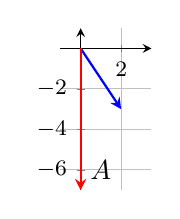
\begin{tikzpicture}[]
\begin{axis}[footnotesize,width=12em
    , axis equal image, axis lines=middle,
    , grid, xmin=-1,xmax=3.5,ymax=1
    ]
    \addplot[blue,quiver={u=2,v=-3},-stealth, thick] coordinates {(0,0)};
    \node[right] at (axis cs:2,-3) {$\xv$};
    \addplot[red,quiver={u=0,v=-7},-stealth, thick] coordinates {(0,0)};
    \node[right] at (axis cs:0,-6) {$A\xv$};
\end{axis}
\end{tikzpicture}%\\[2ex]
}%
For another vector \(\yv=(1,1)\) the product
\begin{equation*}
A\yv=\begin{bmatrix} 3 & 2\\ -2 & 1 \end{bmatrix}
\begin{bmatrix} 1\\1 \end{bmatrix}
=\begin{bmatrix} 3\cdot1+2\cdot1\\ (-2)\cdot1+1\cdot1 \end{bmatrix}
=\begin{bmatrix} 5\\ -1 \end{bmatrix},
\end{equation*}
as illustrated in the second marginal picture.
\marginpar{%
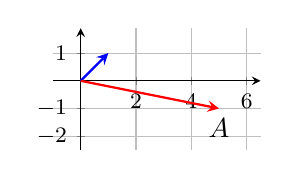
\begin{tikzpicture}[]
\begin{axis}[footnotesize,width=12em
    , axis equal image, axis lines=middle,
    , grid, xmin=-1,xmax=6.5,ymax=1.9,ymin=-2.5
    ]
    \addplot[blue,quiver={u=1,v=1},-stealth, thick] coordinates {(0,0)};
    \node[right] at (axis cs:1,1) {$\yv$};
    \addplot[red,quiver={u=5,v=-1},-stealth, thick] coordinates {(0,0)};
    \node[below] at (axis cs:5,-1) {$A\yv$};
\end{axis}
\end{tikzpicture}%\\[2ex]
}%
Similarly, for the vector \(\zv=(-1,2)\) the product
\begin{equation*}
A\zv=\begin{bmatrix} 3 & 2\\ -2 & 1 \end{bmatrix}
\begin{bmatrix} -1\\2 \end{bmatrix}
=\begin{bmatrix} 3\cdot(-1)+2\cdot2\\ (-2)\cdot(-1)+1\cdot2 \end{bmatrix}
=\begin{bmatrix} 1\\ 4 \end{bmatrix},
\end{equation*}
as illustrated in the third marginal picture.
\marginpar{%
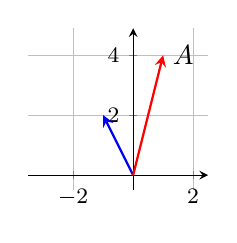
\begin{tikzpicture}[]
\begin{axis}[footnotesize,width=12em
    , axis equal image, axis lines=middle,
    , grid, xmin=-3.5,xmax=2.5,ymax=4.9,ymin=-0.5
    ]
    \addplot[blue,quiver={u=-1,v=2},-stealth, thick] coordinates {(0,0)};
    \node[left] at (axis cs:-1,2) {$\zv$};
    \addplot[red,quiver={u=1,v=4},-stealth, thick] coordinates {(0,0)};
    \node[right] at (axis cs:1,4) {$A\zv$};
\end{axis}
\end{tikzpicture}
}%
Such a geometric interpretation underlies the use of matrix multiplication in video and picture processing, for example.
Such processing employs stretching and shrinking (section~\ref{sec:dmd}), rotations (section~\ref{sec:omr}), among more general transformations (Section~\ref{sec:ilt}).


\begin{example} \label{eg:}
Recall \(I_n\) is the \(n\times n\) \idx{identity matrix}. 
Then the products
\begin{eqnarray*}
I_2\xv&=&\begin{bmatrix} 1&0\\ 0&1 \end{bmatrix}
\begin{bmatrix} 2\\-3 \end{bmatrix}
=\begin{bmatrix} 1\cdot2+0\cdot(-3)\\ 0\cdot2+1\cdot(-3) \end{bmatrix}
=\begin{bmatrix} 2\\ -3 \end{bmatrix},
\\
I_3\bv&=&\begin{bmatrix} 1 & 0 & 0\\ 0 & 1 & 0\\0&0&1 \end{bmatrix}
\begin{bmatrix} 1\\0\\4 \end{bmatrix}
=\begin{bmatrix} 1\cdot1+0\cdot0 + 0\cdot4\\ 0\cdot1 + 1\cdot0 + 0\cdot4\\ 0\cdot1 + 0\cdot0 + 1\cdot4 \end{bmatrix}
=\begin{bmatrix} 1\\0\\4 \end{bmatrix}.
\end{eqnarray*}
That is, and justifying its name of ``identity'', the products with an \idx{identity matrix} give the result that is the vector itself: \(I_2\xv=\xv\) and \(I_3\bv=\bv\)\,.
Multiplication by the identity matrix leaves the vector unchanged (Theorem~\ref{thm:pmmd}).
\end{example}



\begin{example}[\idx{age structured population}] \label{eg:matasp}
% adapted from SACE Math Studies 2012
An ecologist studies an isolated population of a species of animal.
The growth of the population depends primarily upon the females so it is only these that are counted.
The females are grouped into three ages: female pups (in their first year), juvenile females (one year old), and mature females (two years or older).
During the study, the ecologist observes the following happens over the period of a year:
\begin{itemize}
\item  half of the female pups survive and become juvenile females;
\item  one-third of the juvenile females survive and become mature females;
\item  each mature female breeds and produces four female pups;
\item  one-third of the mature females survive to breed in the following year;
\item  female pups and juvenile females do not breed.
\end{itemize}
\begin{enumerate}
\item Let \(x_1\), \(x_2\) and~\(x_3\) be the number of females at the start of a year, of ages zero, one and two+ respectively, and let \(x'_1\), \(x'_2\) and~\(x'_3\) be their number at the start of the next year.
Use the observations to write \(x'_1\), \(x'_2\) and~\(x'_3\) as a function of \(x_1\), \(x_2\) and~\(x_3\)  (this is called a \idx{Markov chain}).
\item Letting vectors \(\xv=(x_1,x_2,x_3)\) and \(\xv'=(x'_1,x'_2,x'_3)\) write down your function as the matrix-vector product \(\xv'=L\xv\) for some matrix~\(L\) (called a \idx{Leslie matrix}).
\item Suppose the ecologist observes the numbers of females at the start of a given year is \(\xv=(60,70,20)\), use your matrix to predict the numbers~\(\xv'\) at the start of the next year.  
Continue similarly to predict the numbers after two years~(\(\xv''\))? and three years~(\(\xv'''\))?
\end{enumerate}

\begin{solution} 
\begin{enumerate}
\item Since mature females breed and produce four female pups, \(x'_1=4x_3\)\,.
Since half of the female pups survive and become juvenile females, \(x'_2=\frac12x_1\)\,.
Since one-third of the juvenile females survive and become mature females, \(\frac13x_2\)~contribute to~\(x'_3\), but additionally one-third of the mature females survive to breed in the following year, so  \(x'_3=\frac13x_2+\frac13x_3\)\,.

\item Writing these equations into vector form
\begin{equation*}
\xv'=\begin{bmatrix} x'_1\\x'_2\\x'_3 \end{bmatrix}
=\begin{bmatrix} 4x_3\\\frac12x_1\\\frac13x_2+\frac13x_3 \end{bmatrix}
=\underbrace{\begin{bmatrix} 0&0&4\\\frac12&0&0\\0&\frac13&\frac13 \end{bmatrix}}_L\xv\,.
\end{equation*}

\item Given the initial numbers of female animals is \(\xv=(60,70,20)\), the number of females after one year is then predicted by the matrix-vector product 
\begin{equation*}
\xv'=L\xv=\begin{bmatrix} 0&0&4\\\frac12&0&0\\0&\frac13&\frac13 \end{bmatrix}
\begin{bmatrix} 60\\70\\20 \end{bmatrix}
=\begin{bmatrix} 80\\30\\30 \end{bmatrix}.
\end{equation*}
That is, the predicted numbers of females are \(80\)~pups, \(30\)~juveniles, and \(30\)~mature.

After a second year the number of females is then predicted by the matrix-vector product \(\xv''=L\xv'\).  Here
\begin{equation*}
\xv''=L\xv'=\begin{bmatrix} 0&0&4\\\frac12&0&0\\0&\frac13&\frac13 \end{bmatrix}\begin{bmatrix} 80\\30\\30 \end{bmatrix}
=\begin{bmatrix} 120\\40\\20 \end{bmatrix}.
\end{equation*}
After a third year the number of females is predicted by the matrix-vector product \(\xv'''=L\xv''\).  Here
\begin{equation*}
\xv'''=L\xv''=\begin{bmatrix} 0&0&4\\\frac12&0&0\\0&\frac13&\frac13 \end{bmatrix}\begin{bmatrix} 120\\40\\20 \end{bmatrix}
=\begin{bmatrix} 80\\60\\20 \end{bmatrix}.
\end{equation*}
\end{enumerate}
\end{solution}
\end{example}







\subsubsection{Matrix-matrix multiplication}

Matrix-vector multiplication explicitly writes the vector in its equivalent form as an \(n\times1\) matrix---a matrix with one column.
Such multiplication immediately generalises to the case of a right-hand matrix with multiple columns.

\begin{example} \label{eg:}
Let matrices
\begin{equation*}
A=\begin{bmatrix} 3 & 2\\ -2 & 1 \end{bmatrix},\quad
B=\begin{bmatrix} 5 & -6 & 4\\ -1 & -3 & -3 \end{bmatrix},
\end{equation*}
then the matrix multiplication~\(AB\) may be done as the matrix~\(A\) multiplying each of the three columns in~\(B\).
That is, in detail write
\begin{eqnarray*}
AB&=&A\begin{bmatrix} 5 & -6 & 4\\ -1 & -3 & -3 \end{bmatrix}
\\&=&A\begin{bmatrix} 5 \V -6 \V 4\\ -1 \V -3 \V -3 \end{bmatrix}
\\&=&\begin{bmatrix} A\begin{bmatrix} 5\\-1 \end{bmatrix} \W
A\begin{bmatrix} -6\\-3 \end{bmatrix} \W
A\begin{bmatrix} 4\\-3 \end{bmatrix} \end{bmatrix}
\\&=&\begin{bmatrix} \begin{bmatrix} 13\\-11 \end{bmatrix} \W
\begin{bmatrix} -24\\9 \end{bmatrix} \W
\begin{bmatrix}6\\-11 \end{bmatrix} \end{bmatrix}
\\&=&\begin{bmatrix}  13& -24&6\\-11 &9&-11\end{bmatrix}.
\end{eqnarray*}
Conversely, the product~\(BA\) cannot be done because if we follow the same procedure
\begin{eqnarray*}
BA&=&B\begin{bmatrix} 3 & 2\\ -2 & 1 \end{bmatrix}
\\&=&B\begin{bmatrix} \begin{bmatrix} 3 \\ -2 \end{bmatrix}\W 
\begin{bmatrix} 2 \\ 1 \end{bmatrix} \end{bmatrix}
\\&=&\begin{bmatrix} B\begin{bmatrix} 3 \\ -2 \end{bmatrix}\W 
B\begin{bmatrix} 2 \\ 1 \end{bmatrix} \end{bmatrix},
\end{eqnarray*}
and neither of these matrix-vector products can be done as, for example,
\begin{equation*}
B\begin{bmatrix} 3 \\ -2 \end{bmatrix}
=\begin{bmatrix} 5 & -6 & 4\\ -1 & -3 & -3 \end{bmatrix}
\begin{bmatrix} 3 \\ -2 \end{bmatrix}
\end{equation*}
the number of columns of the left matrix is not equal to the number of elements of the vector on the right.
Hence the product~\(BA\) is not defined.
\end{example}




\begin{example} \label{eg:}
Let matrices
\begin{equation*}
C=\begin{bmatrix} -4 & -1\\ -4 & -1\\ 1 & 4 \end{bmatrix},\quad
D=\begin{bmatrix} -2 & -1 & -3\\ 1 & 3 & 0 \end{bmatrix}.
\end{equation*}
Compute, if possible, \(CD\) and~\(DC\); compare these products.
\begin{solution} 
\begin{itemize}
\item On the one hand,
\begin{eqnarray*}
CD&=&C\begin{bmatrix} -2 & -1 & -3\\ 1 & 3 & 0 \end{bmatrix}
\\&=&\begin{bmatrix} C\begin{bmatrix} -2\\1 \end{bmatrix}\W
C\begin{bmatrix} -1\\3 \end{bmatrix}\W
C\begin{bmatrix} -3\\0 \end{bmatrix}
 \end{bmatrix}
\\&=&\begin{bmatrix} 7&1&12\\7&1&12\\2&11&-3 \end{bmatrix}.
\end{eqnarray*}

\item Conversely,
\begin{eqnarray*}
DC&=&D\begin{bmatrix} -4 & -1\\ -4 & -1\\ 1 & 4 \end{bmatrix}
\\&=&\begin{bmatrix}  D\begin{bmatrix} -4\\-4\\1 \end{bmatrix}\W
D\begin{bmatrix} -1\\-1\\4 \end{bmatrix}
\end{bmatrix}
\\&=&\begin{bmatrix} 9&-9\\-16&-4 \end{bmatrix}.
\end{eqnarray*}
\end{itemize}
Interestingly, \(CD\neq DC\)\,.
\end{solution}
\end{example}


\begin{definition}[matrix product] \label{def:matprod}
  Let matrix~\(A\) be \(m\times n\), and matrix \(B\) be \(n\times p\), then the \bfidx{matrix product} \(C=AB\) is the \(m\times p\) matrix whose \((i,j)\)th~entry is
\begin{equation*}
c_{ij}=a_{i1}b_{1j}+a_{i2}b_{2j}+\cdots+a_{in}b_{nj}\,.
\end{equation*}
\end{definition}

This formula looks like a dot product of two vectors (\ref{def:dotprod}): indeed we do use that the expression for the \((i,j)\)th~entry is the dot product of the \(i\)th~row of~\(A\) and the \(j\)th~column of~\(B\) as illustrated by
\begin{equation*}
\begin{bmatrix} a_{11}&a_{12}&\cdots&a_{1n}
\\\vdots&\vdots&&\vdots
\\\rlap{\color{blue}\hspace{-0.2em}\framebox{\phantom{\rule{8.7em}{1ex}}}}
a_{i1}&a_{i2}&\cdots&a_{in}
\\\vdots&\vdots&&\vdots
\\a_{m1}&a_{m2}&\cdots&a_{mn} \end{bmatrix}
\begin{bmatrix} b_{11}&\cdots&b_{1j}&\cdots&b_{1p}
\\b_{21}&\cdots&b_{2j}&\cdots&b_{2p}
\\\vdots&&\vdots&&\vdots
\\b_{n1}&\cdots&
\rlap{\color{blue}\hspace{-0.25em}\smash{\framebox{\phantom{\rule[-0.5ex]{1em}{12ex}}}}}
b_{nj}&\cdots&b_{np} \end{bmatrix}.
\end{equation*}
As seen in the examples, although the two matrices~\(A\) and~\(B\) may be of different sizes, the number of columns of~\(A\) must equal the number of rows of~\(B\) in order for the product~\(AB\) to be defined.

\begin{example} \label{eg:}
Matrix multiplication leads to powers of a square matrix.
Let matrix
\begin{equation*}
A=\begin{bmatrix} 3&2\\-2&1 \end{bmatrix},
\end{equation*}
then by~\(A^2\) we mean the product
\begin{equation*}
AA=\begin{bmatrix} 3&2\\-2&1 \end{bmatrix}\begin{bmatrix} 3&2\\-2&1 \end{bmatrix}=\begin{bmatrix} 5&8\\-8&-3 \end{bmatrix},
\end{equation*}
and by~\(A^3\) we mean the product
\begin{equation*}
AAA=AA^2=\begin{bmatrix} 5&8\\-8&-3 \end{bmatrix}\begin{bmatrix} 3&2\\-2&1 \end{bmatrix}
=\begin{bmatrix} -1&18\\-18&-19 \end{bmatrix},
\end{equation*}
and so on.
\end{example}

In general, for an \(n\times n\) square matrix~\(A\) and a positive integer exponent~\(p\) we define the \bfidx{matrix power}
\begin{equation*}
A^p=\underbrace{AA\cdots A}_{p\text{ factors}}.
\end{equation*}
The matrix powers~\(A^p\) are also \(n\times n\) square matrices.


\begin{example}[age structured ecology] \label{eg:poppred}
Matrix powers occur naturally in modelling populations by ecologists such as the animals of Example~\ref{eg:matasp}.
Recall that given the numbers of female pups, juveniles and mature aged formed into a vector \(\xv=(x_1,x_2,x_3)\), the number in each age one year later  (indicated here by a dash) is \(\xv'=L\xv\) for \idx{Leslie matrix}
\begin{equation*}
L=\begin{bmatrix} 0&0&4\\\frac12&0&0\\0&\frac13&\frac13 \end{bmatrix}.
\end{equation*}
Hence the number in each age category two years later (indicated here by two dashes) is
\begin{equation*}
\xv''=L\xv'=L(L\xv)=(LL)\xv=L^2\xv\,,
\end{equation*}
provided that matrix multiplication is associative (Theorem~\ref{thm:pmma}) to enable us to write \(L(L\xv)=(LL)\xv\)\,.
Then the matrix square
\begin{equation*}
L^2=\begin{bmatrix} 0&0&4\\\frac12&0&0\\0&\frac13&\frac13 \end{bmatrix}\begin{bmatrix} 0&0&4\\\frac12&0&0\\0&\frac13&\frac13 \end{bmatrix}
=\begin{bmatrix} 0&\frac43&\frac43\\0&0&2\\\frac16&\frac19&\frac19 \end{bmatrix}.
\end{equation*}
Continuing to use such associativity, 
the number in each age category three years later (indicated here by threes dashes) is
\begin{equation*}
\xv'''=L\xv''=L(L^2\xv)=(LL^2)\xv=L^3\xv\,,
\end{equation*}
where the matrix cube
\begin{equation*}
L^3=LL^2=\begin{bmatrix} 0&0&4\\\frac12&0&0\\0&\frac13&\frac13 \end{bmatrix}\begin{bmatrix} 0&\frac43&\frac43\\0&0&2\\\frac16&\frac19&\frac19 \end{bmatrix}
=\begin{bmatrix} \frac23&\frac49&\frac49\\ 0&\frac23&\frac23\\  \frac1{18}&\frac1{27}&\frac{19}{27}\end{bmatrix}.
\end{equation*}
That is, the powers of the Leslie matrix help predict what happens two, three, or more years into the future.
\end{example}





\subsubsection{The transpose of a matrix}

The operations so far defined for matrices correspond directly to analogous operations for real numbers.
The transpose has no corresponding analogue.
At first mysterious, the transpose occurs frequently---often due to it linking the dot product of vectors with matrix multiplication.
The transpose also reflects symmetry in applications (Chapter~\ref{ch:eesm}), such as Newton's law that every action has an equal and opposite reaction.

\begin{example} \label{eg:mattrans}
Let matrices
\begin{equation*}
A=\begin{bmatrix} -4 & 2\\ -3 & 4\\ -1 & -7 \end{bmatrix},\quad
B=\begin{bmatrix} 2 & 0 & -1 \end{bmatrix},\quad
C=\begin{bmatrix} 1 & 1 & 1\\ -1 & -3 & 0\\ 2 & 3 & 2 \end{bmatrix}.
\end{equation*}
Then obtain the transpose of each of these three matrices by writing each of their rows as columns, in order:
\begin{equation*}
\tr A=\begin{bmatrix} -4 & -3 & -1\\ 2 & 4 & -7 \end{bmatrix},\quad
\tr B=\begin{bmatrix} 2\\ 0\\ -1 \end{bmatrix},\quad
\tr C=\begin{bmatrix} 1 & -1 & 2\\ 1 & -3 & 3\\ 1 & 0 & 2 \end{bmatrix}.
\end{equation*}
\end{example}

These examples illustrate the following definition. 
\begin{definition}[transpose] \label{def:mattran}
The \bfidx{transpose} of an \(m\times n\) matrix~\(A\) is the \(n\times m\) matrix, denoted~\(\tr A\), obtained by writing the \(i\)th~row of~\(A\) as the \(i\)th~column of~\(\tr A\), or equivalently by writing the \(j\)th~column of~\(A\) to be the \(j\)th~row of~\(\tr A\).
That is, if \(B=\tr A\), then \(b_{ij}=a_{ji}\).
\end{definition}


\begin{example}[transpose and dot product] \label{eg:trdp}
Consider two vectors in~\(\RR^n\), say \(\uv=(\hlist un)\) and \(\vv=(\hlist vn)\); that is,
\begin{equation*}
\uv=\begin{bmatrix} u_1\\u_2\\\vdots\\u_n \end{bmatrix},\quad
\vv=\begin{bmatrix} v_1\\v_2\\\vdots\\v_n \end{bmatrix}.
\end{equation*}
Then the dot product between the two vectors
\begin{eqnarray*}
\uv\cdot\vv&=&u_1v_1+u_2v_2+\cdots+u_nv_n \quad(\text{Defn.~\ref{def:dotprod}})
\\&=&\begin{bmatrix} u_1&u_2&\cdots&u_n \end{bmatrix}
\begin{bmatrix} v_1\\v_2\\\vdots\\v_n \end{bmatrix}\quad(\text{matrix mult.})
\\&=&\tr{\begin{bmatrix} u_1\\u_2\\\vdots\\u_n \end{bmatrix}}
\begin{bmatrix} v_1\\v_2\\\vdots\\v_n \end{bmatrix}\quad(\text{matrix transpose})
\\&=&\tr{\uv}\vv\,.
\end{eqnarray*}
Subsequent sections and chapters often use this identity, that \(\uv\cdot\vv=\tr{\uv}\vv\)\,.
\end{example}


\begin{definition}[symmetry] \label{def:matsym}
A matrix~\(A\) is a \bfidx{symmetric matrix} if \(\tr A=A\)\,; that is, if the matrix is equal to its \idx{transpose}.
\end{definition}

A symmetric matrix must be a square matrix---as otherwise the sizes of \(A\) and~\(\tr A\) would be different and so the matrices could not be equal.


\begin{example} \label{eg:}
None of the three matrices in Example~\ref{eg:mattrans} are symmetric: the first two matrices are not square so cannot be symmetric, and the third \(C\neq\tr C\).  
The following matrix is symmetric:
\begin{equation*}
D=\begin{bmatrix} 2 & 0 & 1\\ 0 & -6 & 3\\ 1 & 3 & 4  \end{bmatrix}
=\tr D.
\end{equation*}
When is the following general \(2\times2\) matrix symmetric?
\begin{equation*}
E=\begin{bmatrix} a&b\\c&d \end{bmatrix}.
\end{equation*}
\begin{solution} 
Consider the transpose
\begin{equation*}
\tr E=\begin{bmatrix} a&c\\b&d \end{bmatrix}
\quad\text{compared with }
E=\begin{bmatrix} a&b\\c&d \end{bmatrix}.
\end{equation*}
The top-left and bottom-right elements are always the same.
The top-right and bottom-left elements will be the same if and only if~(iff) \(b=c\).
That is, the \(2\times 2\) matrix~\(E\) is symmetric iff \(b=c\)\,.
\end{solution}
\end{example}

Symmetric matrices of note are the \(n\times n\) \idx{identity matrix} and \(n\times n\) \idx{zero matrix}, \(I_n\) and~\(O_n\).



\subsubsection{Compute in \script}

\script\ empowers us to compute all these operations quickly, especially for the large problems found in applications: after all, Matlab is an abbreviation of \emph{Mat}rix \emph{Lab}oratory.
Table~\ref{tbl:mtlbops} summarises the \script\ version of the operations introduced so far, and used in subsequent sections.

\begin{table}
\caption{As well as the basics of \script\ listed in Table~\ref{tbl:mtlbpre} and~\ref{tbl:mtlbbasics},  we need these matrix operations.\index{Matlab|textbf}\index{Octave|textbf}} \label{tbl:mtlbops}
\hrule
\begin{minipage}{\linewidth}
\begin{itemize}
\item \index{size()@\texttt{size()}}\verb|size(A)| returns the number of rows and columns of matrix~\(A\): if \(A\) is \(m\times n\), then \verb|size(A)| returns \(\begin{bmatrix} m&n \end{bmatrix}\).
\item \verb|A(i,j)| is the \((i,j)\)th entry of a matrix~\(A\), \verb|A(:,j)|~is the \(j\)th~column, \verb|A(i,:)|~is the \(i\)th~row; either to use the value(s) or to assign value(s).
\item \index{+,-,*@\texttt{+,-,*}}\verb|+,-,*| is matrix\slash vector\slash scalar addition, subtraction, and multiplication, but only provided the sizes of the two operands are compatible.
%\item As well as enclosing subscripts, parentheses,~\verb|()|, control the order of evaluation of a complicated expression.
\item \verb|A^p| for scalar~\(p\) computes the \(p\)th~power of square matrix~\(A\) (in contrast to~\verb|A.^p| which  computes the \(p\)th~power of \emph{each element} of~\(A\), Table~\ref{tbl:mtlbbasics}).
\item The character single \idx{quote},~\verb|A'|, \idx{transpose}s the matrix~\(A\).
\item Predefined matrices include:
\begin{itemize}
\item \index{zero matrix}\index{zeros()@\texttt{zeros()}}\verb|zeros(m,n)| is the \idx{zero matrix}~\(O_{m\times n}\);
\item \index{eye()@\texttt{eye()}}\verb|eye(m,n)|~is \(m\times n\) `\idx{identity matrix}'~\(I_{m\times n}\);
\item \index{ones matrix}\index{ones()@\texttt{ones()}}\verb|ones(m,n)| is the \(m\times n\) matrix where all entries are one;
\item \index{random matrix}\index{randn()@\texttt{randn()}}\verb|randn(m,n)|~is a \(m\times n\) matrix with random entries (distributed Normally, mean zero, standard deviation one).
\end{itemize}
A single argument gives the \idx{square matrix} version: 
\begin{itemize}
\item \index{zero matrix}\verb|zeros(n)| is~\(O_n=O_{n\times n}\); 
\item \verb|eye(n)|~is the \(n\times n\) \idx{identity matrix} \(I_n=I_{n\times n}\);  
\item \verb|ones(n)| is the \(n\times n\) matrix of all ones;
\item \index{random matrix}\verb|randn(n)|~is an \(n\times n\) matrix with random entries.
\end{itemize}
With no argument, these functions return the corresponding scalar: for example, \verb|randn|~computes a single random number.
\item Very large and small magnitide numbers are printed in \script\ like the following: 
\begin{itemize}
\item \verb|4.852e+08| denotes the large \(4.852\cdot10^8\); whereas 
\item \verb|3.469e-16| denotes the small \(3.469\cdot10^{-16}\).
\end{itemize}
\end{itemize}
\end{minipage}
\hrule
\end{table}

\paragraph{Matrix size and elements}
Let the matrix
\begin{equation*}
A=\begin{bmatrix} 0 & 0 & -2 & -11 & 5\\ 0 & 1 & -1 & 11 & -8\\ -4 & 2 & 10 & 2 & -3 \end{bmatrix}.
\end{equation*}
We readily see this is a \(3\times5\) matrix, but to check that \script\ agrees, execute the following in \script: \index{size}
\begin{verbatim}
A=[0 0 -2 -11  5
   0 1 -1  11 -8
  -4 2 10   2 -3]
size(A)
\end{verbatim}
\setbox\ajrqrbox\hbox{\qrcode{% matrix elements
A=[0 0 -2 -11  5
   0 1 -1  11 -8
  -4 2 10   2 -3]
size(A)
A(2,4)
A(:,5)
A(1,:)
A(2,4)=9
A(:,5)=[2;-3;1]
A(1,:)=[1 2 3 4 5]
}}%
\marginpar{\usebox{\ajrqrbox\\[2ex]}}%
The answer, ``\verb|3  5|'', confirms \(A\) is \(3\times5\).
\script\ accesses individual elements, rows and columns.
For example, execute each of the following:
\begin{itemize}
\item \verb|A(2,4)| gives~\(a_{24}\) which here is~\(11\);
\item \verb|A(:,5)| is the the fifth \idx{column vector}, here \(\begin{bmatrix} 5\\ -8\\ -3 \end{bmatrix}\);
\item \verb|A(1,:)| is the first row, here \(\begin{bmatrix} 0 & 0 & -2 & -11 & 5 \end{bmatrix}\).
\end{itemize}
One may also use these constructs to change the elements in matrix~\(A\): for example, executing
\verb|A(2,4)=9| changes matrix~\(A\) to
\begin{verbatim}
A =
     0     0    -2   -11     5
     0     1    -1     9    -8
    -4     2    10     2    -3
\end{verbatim}
then \verb|A(:,5)=[2;-3;1]| changes matrix~\(A\) to
\begin{verbatim}
A =
     0     0    -2   -11     2
     0     1    -1     9    -3
    -4     2    10     2     1
\end{verbatim}
whereas \verb|A(1,:)=[1 2 3 4 5]| changes matrix~\(A\) to
\begin{verbatim}
A =
     1     2     3     4     5
     0     1    -1     9    -3
    -4     2    10     2     1
\end{verbatim}


\paragraph{Matrix addition and subtraction}
To illustrate further operations let's use some random matrices generated by \script: you will generate different matrices to the following, but the operations will work the same.
Table~\ref{tbl:mtlbops} mentions that \verb|randn(m,n)| generates a random matrix so execute say
\begin{verbatim}
A=randn(4)
B=randn(4)
C=randn(4,2)
\end{verbatim}
and obtain matrices such as \twodp
\setbox\ajrqrbox\hbox{\qrcode{% matrix add and subtract
A=randn(4)
B=randn(4)
C=randn(4,2)
A+B
A-B
(A+B)-(B+A)
B+C
}}%
\marginpar{\usebox{\ajrqrbox\\[2ex]}}%
\begin{verbatim}
A =
  -1.31   2.07   0.08   2.05
   1.25  -1.35  -1.00   1.94
   1.08   1.79  -0.99   0.93
   1.34  -0.99  -0.23  -0.22
B =
   1.21  -0.46   0.09   0.58
   1.67  -1.96   1.26   1.93
   0.24  -0.46   2.77  -0.59
   0.03  -0.28  -0.76   0.13
C =
   1.14   0.85
  -0.48   0.17
   0.37  -0.64
   0.62  -1.17
\end{verbatim}
Then \verb|A+B| gives here the sum\index{addition}\index{sum}
\begin{verbatim}
ans =
  -0.10   1.62   0.17   2.63
   2.92  -3.31   0.26   3.87
   1.31   1.33   1.78   0.34
   1.37  -1.27  -0.99  -0.09
\end{verbatim}
and \verb|A-B| the difference\index{subtraction}\index{difference}
\begin{verbatim}
ans =
  -2.52   2.53  -0.01   1.46
  -0.41   0.62  -2.25   0.01
   0.84   2.26  -3.76   1.52
   1.31  -0.71   0.53  -0.35
\end{verbatim}
You could check that \verb|B+A| gives the same matrix as \verb|A+B| (Theorem~\ref{thm:pasma}) by seeing that their difference is the \(3\times5\) zero matrix: execute \verb|(A+B)-(B+A)| (the parentheses control the order of evaluation).
However, expressions such as \verb|B+C| and \verb|A-C| give an error, because the matrices are of incompatible sizes, reported by Matlab as\index{Error using}
\begin{verbatim}
Error using  + 
Matrix dimensions must agree. 
\end{verbatim}
or reported by Octave as\index{error: operator}
\begin{verbatim}
error: operator +: nonconformant arguments 
\end{verbatim}


\paragraph{Scalar multiplication of matrices}
In \script\ the asterisk indicates multiplication.
Scalar multiplication can be done either way around.
For example, generate a random \(2\times 4\) matrix~\(A\) and compute \(2A\) and~\(A\frac1{10}\).
These commands 
\begin{verbatim}
A=randn(4,3)
2*A
A*0.1
\end{verbatim}
\setbox\ajrqrbox\hbox{\qrcode{% scalar multiplication et al
A=randn(4,3)
2*A
A*0.1
A+3
2*A-5
}}%
\marginpar{\usebox{\ajrqrbox\\[2ex]}}%
might give the following \twodp
\begin{verbatim}
A =
   0.82   2.54  -0.98
   2.30   0.05   2.63
  -1.45   2.15   0.89
  -2.58  -0.09  -0.55

>> 2*A
ans =
   1.64   5.07  -1.97
   4.61   0.10   5.25
  -2.90   4.30   1.77
  -5.16  -0.18  -1.11

>> A*0.1
ans =
   0.08   0.25  -0.10
   0.23   0.00   0.26
  -0.15   0.21   0.09
  -0.26  -0.01  -0.06
\end{verbatim}
Division by a scalar is also defined in \script\ and means multiplication by the reciprocal; for example, the product~\verb|A*0.1| could equally well be computed as~\verb|A/10|.

In mathematical algebra we would not normally accept statements such as \(A+3\) or \(2A-5\) because addition and subtraction with matrices has only been defined between matrices of the same size.\footnote{Although in some contexts such mathematical expressions are routinely accepted, be careful of their meaning.}
However, \script\ usefully extends addition and subtraction so that \verb|A+3| and \verb|2*A-5| mean add three to \emph{every} element of~\(A\) and subtract five from \emph{every} element of~\(2A\). 
For example, with the above random \(4\times3\) matrix~\(A\),
\begin{verbatim}
>> A+3
ans =
   3.82   5.54   2.02
   5.30   3.05   5.63
   1.55   5.15   3.89
   0.42   2.91   2.45

>> 2*A-5
ans =
   -3.36    0.07   -6.97
   -0.39   -4.90    0.25
   -7.90   -0.70   -3.23
  -10.16   -5.18   -6.11
\end{verbatim}
This last computation illustrates that in any expression the operations of multiplication and division are performed before additions and subtractions---as normal in mathematics.


\paragraph{Matrix multiplication}
In \script\ the asterisk also invokes matrix-matrix and matrix-vector multiplication.
For example, generate and multiply two random matrices say of size \(3\times4\) and \(4\times 3\) \twodp\ with
\begin{verbatim}
A=randn(3,4)
B=randn(4,2)
C=A*B
\end{verbatim}
\setbox\ajrqrbox\hbox{\qrcode{% scalar multiplication et al
A=randn(3,4)
B=randn(4,2)
C=A*B
A(1,:)*B(:,1)
[A*B(:,1) A*B(:,2)]
B*A
}}%
\marginpar{\usebox{\ajrqrbox\\[2ex]}}%
might give the following result
\begin{verbatim}
A =
  -0.02   1.31  -0.74  -0.49
  -0.36  -1.30  -0.23   0.41
  -0.88  -0.34   0.28  -0.99

B =
  -1.32  -0.79
   0.71   1.48
  -0.48   2.79
   1.40  -0.41

>> C=A*B
C =
   0.62   0.10
   0.24  -2.44
  -0.60   1.38
\end{verbatim}
Without going into excruciating arithmetic detail this product is hard to check.
However, we can check several things such as the first row of~\(A\) times the first column of~\(B\) gives~\(c_{11}\) by computing \verb|A(1,:)*B(:,1)| and seeing it does give~\(0.62\) as required.
Also check that the two columns of~\(C\) may be viewed as the two matrix-vector products \(A\bv_1\) and~\(A\bv_2\) by comparing~\(C\) with \verb|[A*B(:,1) A*B(:,2)]| and seeing they are the same.

Recall that in a matrix product the number of columns of the left matrix have to be the same as the number of rows of the right matrix.
\script\ gives an error message if this is not the case, such as occurs  upon asking it to compute~\verb|B*A| when Matlab reports\index{Error using}
\begin{verbatim}
Error using  * 
Inner matrix dimensions must agree.
\end{verbatim}
and Octave reports\index{error: operator}
\begin{verbatim}
error: operator *: nonconformant arguments
\end{verbatim}

The caret symbol computes matrix powers in \script, such as the cube~\verb|A^3|, but it only makes sense and works for square matrices~\(A\).\footnote{We define matrix powers for only integer power. \script\ will compute the power of a square matrix for any real\slash complex exponent, but its meaning involves matrix exponentials and logarithms that we do not explore here.}
For example, if matrix~\(A\) was \(3\times4\)\,, then \(A^2=AA\) would involve multiplying a \(3\times4\) matrix by a \(3\times4\) matrix: since the number of columns of the left~\(A\) is not the same as the number of rows of the right~\(A\) such a multiplication is not allowed.



\paragraph{The transpose and symmetry}
In \script\ the single apostrophe denotes matrix \idx{transpose}.
For example, see it transpose a couple of random matrices with
\begin{verbatim}
A=randn(3,4)
B=randn(4,2)
A'
B'
\end{verbatim}
\setbox\ajrqrbox\hbox{\qrcode{% scalar multiplication et al
A=randn(3,4)
B=randn(4,2)
A'
B'
(A*B)'-B'*A'
C=randn(3)
C=C+C'
C-C'
}}%
\marginpar{\usebox{\ajrqrbox\\[2ex]}}%
giving here for example \twodp
\begin{verbatim}
A =
   0.80   0.30  -0.12  -0.57
   0.07  -0.51  -0.81   1.95
   0.29  -0.10   0.17   0.70
B =
  -0.71  -0.34
  -0.33  -0.73
   1.11  -0.21
   0.41   0.33

>> A'
ans =
   0.80   0.07   0.29
   0.30  -0.51  -0.10
  -0.12  -0.81   0.17
  -0.57   1.95   0.70

>> B'
ans =
  -0.71  -0.33   1.11   0.41
  -0.34  -0.73  -0.21   0.33
\end{verbatim}
One can do further operations after the transposition, such as checking the multiplication rule that \(\tr{(AB)}=\tr B\tr A\) (Theorem~\ref{thm:potd}) by verifying \verb|(A*B)'-B'*A'| is the zero matrix, here~\(O_{2\times3}\).

You can generate a symmetric matrix by adding a square matrix to its transpose (Theorem~\ref{thm:potf}): for example, generate a random square matrix by first \verb|C=randn(3)| then \verb|C=C+C'| makes a random symmetric matrix such as the following \twodp
\begin{verbatim}
>> C=randn(3)
C =
  -0.33   0.65  -0.62
  -0.43  -2.18  -0.28
   1.86  -1.00  -0.52

>> C=C+C'
C =
  -0.65   0.22   1.24
   0.22  -4.36  -1.28
   1.24  -1.28  -1.04

>> C-C'
ans =
   0.00   0.00   0.00
   0.00   0.00   0.00
   0.00   0.00   0.00
\end{verbatim}
That the resulting matrix~\(C\) is symmetric is checked by this last step which computes the difference between~\(C\) and~\(\tr C\) and confirming the difference is zero. 






\subsection{Familiar algebraic properties of matrix operations}
\label{sec:fapmo}

Almost all of the familiar algebraic properties of scalar addition, subtraction and multiplication---namely commutativity, associativity and distributivity---hold for matrix addition, subtraction and multiplication.

The one outstanding exception is that matrix multiplication is \emph{not} commutative: for matrices~\(A\) and~\(B\) the products~\(AB\) and~\(BA\) are usually not equal.
We are used to non-commutativity in life.
For example, when you go home, to enter your house you first open the door, second walk in, and third close the door. 
You cannot swap the order and try to walk in before opening the door---the operations do not commute.
Similarly, for another example, I often teach classes on the third floor of a building next to my office: after finishing classes, first I walk downstairs to ground level, and second I cross the road to my office.
If I try to cross the road before going downstairs, then the force of gravity has something very painful to say about the outcome---the operations do not commute.
Similar to these analogues, the order of matrix multiplication makes a difference to the result.


\begin{theorem}[Properties of addition and scalar multiplication] \label{thm:pasm}
Let matrices \(A\), \(B\) and~\(C\) be of the same size, and let \(c\) and~\(d\) be scalars.  Then:
\begin{enumerate}
\item\label{thm:pasma} \(A+B=B+A\) (commutativity of addition);
\item \((A+B)+C=A+(B+C)\) (associativity of addition);
\item \(A\pm O=A=O+A\);
\item \(c(A\pm B)=cA\pm cB\) (distributivity over matrix addition);
\item \((c\pm d)A=cA\pm dA\) (distributivity over scalar addition);
\item \(c(dA)=(cd)A\) (associativity of scalar multiplication);
\item \(1A=A\)\,; and 
\item \(0A=O\)\,.
\end{enumerate}
\end{theorem}

\begin{proof}
The proofs directly match those of the corresponding vector properties and are set as exercises.
\end{proof}



\begin{example}[geometry of associativity]
Many properties of matrix multiplication have a useful geometric interpretation such as that discussed for matrix-vector products.
Recall the earlier Example~\ref{eg:poppred} invoked the associativity Theorem~\ref{thm:pmma}.
For another example, consider the two matrices and vector
\begin{equation*}
A=\begin{bmatrix} 1&1\\1&0 \end{bmatrix},\quad
B=\begin{bmatrix} 2&0\\2&-1 \end{bmatrix},\quad
\xv=\begin{bmatrix} 1\\1 \end{bmatrix}.
\end{equation*}
Now the transform \(\xv'=B\xv=(2,1)\), and then transforming with~\(A\) gives \(\xv''=A\xv'=A(B\xv)=(3,2)\), as illustrated in the margin.
\marginpar{%
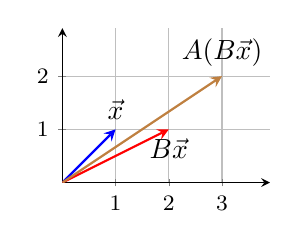
\begin{tikzpicture}[]
\begin{axis}[footnotesize,width=12em
    , axis equal image, axis lines=middle,
    , grid,xmin=0,xmax=3.9,ymax=2.9
    ]
    \addplot[blue,quiver={u=1,v=1},-stealth, thick] coordinates {(0,0)};
    \node[above] at (axis cs:1,1) {$\vec x$};
    \addplot[red,quiver={u=2,v=1},-stealth, thick] coordinates {(0,0)};
    \node[below] at (axis cs:2,1) {$B\vec x$};
    \addplot[brown,quiver={u=3,v=2},-stealth, thick] coordinates {(0,0)};
    \node[above] at (axis cs:3,2) {$A(B\vec x)$};
\end{axis}
\end{tikzpicture}
}%
This is the same results as forming the product
\begin{equation*}
AB=\begin{bmatrix} 1&1\\1&0 \end{bmatrix} 
\begin{bmatrix} 2&0\\2&-1 \end{bmatrix}
=\begin{bmatrix} 4&-1\\2&0 \end{bmatrix}
\end{equation*}
and then computing \((AB)\xv=(3,2)\) as also illustrated in the margin.
\marginpar{%
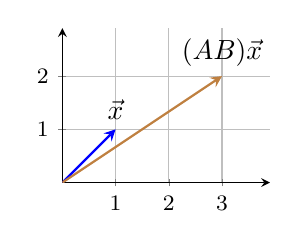
\begin{tikzpicture}[]
\begin{axis}[footnotesize,width=12em
    , axis equal image, axis lines=middle,
    , grid,xmin=0,xmax=3.9,ymax=2.9
    ]
    \addplot[blue,quiver={u=1,v=1},-stealth, thick] coordinates {(0,0)};
    \node[above] at (axis cs:1,1) {$\vec x$};
%    \addplot[red,quiver={u=2,v=1},-stealth, thick] coordinates {(0,0)};
%    \node[below] at (axis cs:2,1) {$B\vec x$};
    \addplot[brown,quiver={u=3,v=2},-stealth, thick] coordinates {(0,0)};
    \node[above] at (axis cs:3,2) {$(AB)\vec x$};
\end{axis}
\end{tikzpicture}
}%
Such associativity asserts that \(A(B\xv)=(AB)\xv\)\,: that is, the geometric transform of~\xv\ by matrix~\(B\) followed by the transform of matrix~\(A\) is the same result as just transforming by the matrix formed from the product~\(AB\)---as assured by Theorem~\ref{thm:pmma}.
\end{example}



\begin{theorem}[properties of matrix multiplication] \label{thm:pmm}
Let matrices \(A\), \(B\) and~\(C\) be of sizes such that the following expressions are defined, and let \(c\)~be a scalar, then:
\begin{enumerate}
\item\label{thm:pmmb} \(A(B\pm C)=AB\pm AC\) (distributivity of matrix multiplication);
\item\label{thm:pmmbb} \((A\pm B)C=AC\pm BC\) (distributivity of matrix multiplication);
\item\label{thm:pmma} \(A(BC)=(AB)C\) (associativity of matrix multiplication);
\item\label{thm:pmmc} \(c(AB)=(cA)B=A(cB)\);
\item\label{thm:pmmd} \(I_mA=A=AI_n\) for \(m\times n\) matrix~\(A\) (multiplicative identity);
\item\label{thm:pmme} \(O_mA=O_{m\times n}=AO_n\)  for \(m\times n\) matrix~\(A\);
\item\label{thm:pmmg} \(A^pA^q=A^{p+q}\), \((A^p)^q=A^{pq}\) and~\((cA)^p=c^pA^p\) for square~\(A\) and for positive integers~\(p\) and~\(q\).\footnote{Generically, these exponent properties hold for all scalar~\(p\) and~\(q\), although we have to be very careful with non-integer exponents.}
\end{enumerate}
\end{theorem}

\begin{proof} 
Let's document a few proofs, others are exercises.
\begin{description}
\item[\ref{thm:pmmb}]
The direct proof involves some long expressions involving the entries of \(m\times n\) matrix~\(A\), and \(n\times p\) matrices~\(B\) and~\(C\).
Let \((\cdot)_{ij}\) denote the \((i,j)\)th~entry of whatever matrix expression is inside the parentheses.
By Definition~\ref{def:matprod} of matrix multiplication
\begin{align*}
&(A(B\pm C))_{ij}
\\&=a_{i1}(B\pm C)_{1j}+a_{i2}(B\pm C)_{2j}+\cdots+a_{in}(B\pm C)_{nj}
\\&\qquad(\text{by definition of matrix addition})
\\&=a_{i1}(b_{1j}\pm c_{1j})+a_{i2}(b_{2j}\pm c_{2j})+\cdots+a_{in}(b_{nj}\pm c_{nj})
\\&\qquad(\text{distributing the scalar multiplications})
\\&=a_{i1}b_{1j}\pm a_{i1}c_{1j}+a_{i2}b_{2j}\pm a_{i2}c_{2j}+\cdots+a_{in}b_{nj}\pm a_{in}c_{nj}
\\&\qquad(\text{upon reordering terms in the sum})
\\&=a_{i1}b_{1j}+a_{i2}b_{2j}+\cdots+a_{in}b_{nj}
\\&\quad{}\pm (a_{i1}c_{1j}+ a_{i2}c_{2j}+\cdots +a_{in}c_{nj})
\\&\qquad(\text{using Definition~\ref{def:matprod} for matrix products})
\\&=(AB)_{ij} \pm (AC)_{ij}\,.
\end{align*}
Since this identity holds for all indices~\(i\) and~\(j\), the matrix identity \(A(B\pm C)=AB\pm AC\) holds, proving Theorem~\ref{thm:pmmb}.


\item[\ref{thm:pmma}] Associativity involves some longer expressions involving the entries of \(m\times n\) matrix~\(A\), \(n\times p\) matrix~\(B\), and \(p\times q\) matrix~\(C\). 
By Definition~\ref{def:matprod} of matrix multiplication
\begin{eqnarray*}
%&\rlap{$(A(BC))_{ij}$}\\
(A(BC))_{ij}&=& a_{i1}(BC)_{1j}+a_{i2}(BC)_{2j}+\cdots+a_{in}(BC)_{nj}
\\&&\quad(\text{then using  Definition~\ref{def:matprod} for }BC)
\\&=&\phantom{{}+{}}a_{i1}(b_{11}c_{1j}+b_{12}c_{2j}+\cdots+b_{1p}c_{pj})
\\&&{}+a_{i2}(b_{21}c_{1j}+b_{22}c_{2j}+\cdots+b_{2p}c_{pj})
\\&&{}+\cdots
\\&&{}+a_{in}(b_{n1}c_{1j}+b_{n2}c_{2j}+\cdots+b_{np}c_{pj})
\\&&{}\quad(\text{distributing the scalar multiplications})
\\&=&\phantom{{}+{}}a_{i1}b_{11}c_{1j}+a_{i1}b_{12}c_{2j}+\cdots+a_{i1}b_{1p}c_{pj}
\\&&{}+a_{i2}b_{21}c_{1j}+a_{i2}b_{22}c_{2j}+\cdots+a_{i2}b_{2p}c_{pj}
\\&&{}+\cdots
\\&&{}+a_{in}b_{n1}c_{1j}+a_{in}b_{n2}c_{2j}+\cdots+a_{in}b_{np}c_{pj}
\\&&{}\quad(\text{reordering the terms---transpose})
\\&=&\phantom{{}+{}}a_{i1}b_{11}c_{1j}+a_{i2}b_{21}c_{1j}+\cdots+a_{in}b_{n1}c_{1j}
\\&&{}+a_{i1}b_{12}c_{2j}+a_{i2}b_{22}c_{2j}+\cdots+a_{in}b_{n2}c_{2j}
\\&&{}+\cdots
\\&&{}+a_{i1}b_{1p}c_{pj}+a_{i2}b_{2p}c_{pj}+\cdots+a_{in}b_{np}c_{pj}
\\&&{}\quad(\text{factoring }c_{1j},c_{2j},\ldots c_{pj})
\\&=&\phantom{{}+{}}(a_{i1}b_{11}+a_{i2}b_{21}+\cdots+a_{in}b_{n1})c_{1j}
\\&&{}+(a_{i1}b_{12}+a_{i2}b_{22}+\cdots+a_{in}b_{n2})c_{2j}
\\&&{}+\cdots
\\&&{}+(a_{i1}b_{1p}+a_{i2}b_{2p}+\cdots+a_{in}b_{np})c_{pj}
\\&&{}\quad(\text{recognising the entries for }(AB)_{ik})
\\&=&(AB)_{i1}c_{1j} +(AB)_{i2}c_{2j} +\cdots +(AB)_{ip}c_{pj}
\\&&{}\quad(\text{again using  Definition~\ref{def:matprod}})
\\&=&((AB)C)_{ij}.
\end{eqnarray*}
Since this identity holds for all indices~\(i\) and~\(j\), the matrix identity \(A(BC)=(AB)C\) holds, proving Theorem~\ref{thm:pmma}.

\item[\ref{thm:pmmg}]
Other proofs develop from previous parts of the theorem.
For example, to establish \(A^pA^q=A^{p+q}\) start from the definition of matrix powers:
\begin{eqnarray*}
A^pA^q&=&\underbrace{AA\cdots A}_{p\text{ times}}
\underbrace{AA\cdots A}_{q\text{ times}}
\\&&\quad(\text{using associativity, Thm.~\ref{thm:pmma}})
\\&=&\underbrace{AA\cdots A}_{p+q\text{ times}}
\\&=&A^{p+q}.
\end{eqnarray*}

\end{description}
\end{proof}



\begin{example} \label{eg:}
Show that \((A+B)^2\neq A^2+2AB+B^2\)  in general.
\begin{solution} 
Consider
\begin{eqnarray*}
(A+B)^2&=& (A+B)(A+B) \quad(\text{matrix power})
\\&=&A(A+B)+B(A+B) \quad(\text{Thm.~\ref{thm:pmmbb}})
\\&=&AA+AB+BA+BB \quad(\text{Thm.~\ref{thm:pmmb}})
\\&=&A^2+AB+BA+B^2 \quad(\text{matrix power}).
\end{eqnarray*}
This expression is only equal to \(A^2+2AB+B^2\) if we can replace \(BA\) by~\(AB\).  
But this requires \(BA=AB\) which is generally not true.
That is, \((A+B)^2= A^2+2AB+B^2\) only if \(BA=AB\)\,.
\end{solution}
\end{example}




\begin{example} \label{eg:}
Show that the matrix \(J=\begin{bmatrix} 0&0&1\\0&1&0\\1&0&0 \end{bmatrix}\) is not a multiplicative identity (despite having ones down a diagonal, this diagonal is the wrong one for an identity).
\begin{solution} 
Among many other ways to show \(J\)~is not a multiplicative identity, let's invoke a general \(3\times3\) matrix
\begin{equation*}
A=\begin{bmatrix} a&b&c\\d&e&f\\g&h&i \end{bmatrix},
\end{equation*}
and evaluate the product
\begin{equation*}
JA=
\begin{bmatrix} 0&0&1\\0&1&0\\1&0&0 \end{bmatrix}
\begin{bmatrix} a&b&c\\d&e&f\\g&h&i \end{bmatrix}
=\cdots
=\begin{bmatrix} g&h&i\\d&e&f\\a&b&c \end{bmatrix}
\neq A\,.
\end{equation*}
Since \(JA\neq A\) then matrix~\(J\) cannot be a multiplicative identity (the multiplicative identity is only when the ones are along the diagonal from top-left to bottom-right).
\end{solution}
\end{example}




\begin{theorem}[properties of transpose] \label{thm:pot}
Let matrices \(A\) and~\(B\) be of sizes such that the following expressions are defined, then:
\begin{enumerate}
\item\label{thm:pota} \(\tr{(\tr A)}=A\);
\item\label{thm:potb} \(\tr{(A\pm B)}=\tr A\pm \tr B\);
\item\label{thm:potc} \(\tr{(cA)}=c(\tr A)\) for any scalar~\(c\);
\item\label{thm:potd} \(\tr{(AB)}=\tr B\tr A\);
\item\label{thm:pote} \(\tr{(A^p)}=(\tr A)^p\) for all positive integer exponents~\(p\);\footnote{With care, this property also holds for all scalar exponents~\(p\).}
\item\label{thm:potf} \(A+\tr A\),  \(\tr AA\) and \(A\tr A\) are symmetric matrices.
\end{enumerate}
\end{theorem}

\begin{proof} 
Let's document a few proofs, others are exercises.
Some proofs use primitive definitions---usually using \((\cdot)_{ij}\) to denote the \((i,j)\)th~entry of whatever matrix expression is inside the parentheses---others invoke earlier proved parts.
\begin{description}
\item[\ref{thm:potb}]
Recall from Definition~\ref{def:mattran} of the transpose that
\begin{eqnarray*}
(\tr{(A\pm B)})_{ij}
&=&(A\pm B)_{ji}
\\&&\quad(\text{by definition of addition})
\\&=&a_{ji}\pm b_{ji}
\\&&\quad(\text{by Defn.~\ref{def:mattran} of transpose})
\\&=&(\tr A)_{ij}\pm(\tr B)_{ij}\,.
\end{eqnarray*}
Since this identity holds for all indices~\(i\) and~\(j\), then \(\tr{(A\pm B)}=\tr A\pm \tr B\) .

\item[\ref{thm:potd}]
The transpose of matrix multiplication is more involved.
Let matrices~\(A\) and~\(B\) be of sizes \(m\times n\) and \(n\times p\) respectively.  Then from Definition~\ref{def:mattran} of the transpose
\begin{align*}
&(\tr{(AB)})_{ij}=(AB)_{ji}
\\&\qquad(\text{by Defn.~\ref{def:matprod} of multiplication})
\\&=a_{j1}b_{1i}+a_{j2}b_{2i}+\cdots+a_{jn}b_{ni}
\\&\qquad(\text{commuting the products})
\\&=b_{1i}a_{j1}+b_{2i}a_{j2}+\cdots+b_{ni}a_{jn}
\\&\qquad(\text{by Defn.~\ref{def:mattran} of  transpose})
\\&=(\tr B)_{i1}(\tr A)_{1j}+(\tr B)_{i2}(\tr A)_{2j}+\cdots+(\tr B)_{in}(\tr A)_{nj}
\\&\qquad(\text{by Defn.~\ref{def:matprod} of multiplication})
\\&=(\tr B\tr A)_{ij}\,.
\end{align*}
Since this identity holds for all indices~\(i\) and~\(j\), then \(\tr{(AB)}=\tr B\tr A\).

\item[\ref{thm:potf}] To prove the second, that \(\tr AA\) is equal to its transpose, we invoke earlier parts.
Consider the transpose 
\begin{eqnarray*}
\tr{(\tr AA)}&=& \tr{(A)}\tr{(\tr A)}\quad(\text{by~\ref{thm:potd}})
\\&=&\tr AA\quad(\text{by~\ref{thm:pota}}).
\end{eqnarray*}
Since \(\tr AA\) equals its transpose, it is symmetric.
\end{description}
\end{proof}








\subsection{Exercises}


\begin{exercise} \label{ex:} 
Consider the following six matrices:
\(A=\begin{bmatrix} -1&3
\\0&-5
\\0&-7 \end{bmatrix}\);
\(B=\begin{bmatrix} -4&-3&-3&1
\\-3&-2&0&-1 \end{bmatrix}\);
\(C=\begin{bmatrix} -3&1 \end{bmatrix}\);
\(D=\begin{bmatrix} 0&6&6&3
\\2&2&0&-5 \end{bmatrix}\);
\(E=\begin{bmatrix} 0&1&1&-2
\\-1&5&4&-1
\\1&-3&7&3
\\-6&-3&0&2 \end{bmatrix}\);
\(F=\begin{bmatrix} 4&1&0
\\-1&1&6
\\-4&5&-2 \end{bmatrix}\).
\begin{enumerate}
\item What is the size of each of these matrices?
\answer{\(A,\ 3\times2\);
\(B,\ 2\times4\);
\(C,\ 1\times2\);
\(D,\ 2\times4\);
\(E,\ 4\times4\);
\(F,\ 3\times3\).}

\item  Which pairs of matrices may be added or subtracted?
\answer{Only \(B\) and~\(D\).}

\item  Which matrix multiplications can be performed between two of the matrices?
\answer{\(AB,\ AD,\ BE,\ CB,\ CD,\ DE,\ E^2,\ FA,\ F^2\).}

\end{enumerate}
\end{exercise}





\begin{exercise} \label{ex:} 
Consider the following six matrices:
\(A=\begin{bmatrix} 3&\tfrac{17}{6}
\\-\tfrac{5}{3}&\tfrac{1}{2}
\\-\tfrac{1}{6}&-\tfrac{1}{6}
\\\tfrac{5}{3}&1 \end{bmatrix}\);
\(B=\begin{bmatrix} \tfrac{7}{6}&\tfrac{1}{3}&\tfrac{17}{3} \end{bmatrix}\);
\(C=\begin{bmatrix} -\tfrac{11}{3}&-\tfrac{7}{3}
\\\tfrac{2}{3}&\tfrac{4}{3}
\\\tfrac{3}{2}&-\tfrac{17}{6} \end{bmatrix}\);
\(D=\begin{bmatrix} 0&-\tfrac{13}{6}&0&\tfrac{13}{3}
\\\tfrac{20}{3}&2&-\tfrac{8}{3}&-\tfrac{7}{2}
\\\tfrac{5}{6}&\tfrac{1}{3}&\tfrac{13}{6}&-\tfrac{16}{3} \end{bmatrix}\);
\(E=\begin{bmatrix} \tfrac{13}{6}&-\tfrac{1}{6}
\\-\tfrac{7}{3}&-5 \end{bmatrix}\);
\(F=\begin{bmatrix} -\tfrac{1}{3}
\\\tfrac{13}{3} \end{bmatrix}\).
\begin{enumerate}
\item What is the size of each of these matrices?
\answer{\(A,\ 4\times2\);
\(B,\ 1\times3\);
\(C,\ 3\times2\);
\(D,\ 3\times4\);
\(E,\ 2\times2\);
\(F,\ 2\times1\).}

\item  Which pairs of matrices may be added or subtracted?
\answer{None.}

\item  Which matrix multiplications can be performed between two of the matrices?
\answer{\(AE,\ AF,\ BC,\ BD,\ CE,\ CF,\ DA,\ E^2,\ EF,\ FB\).}

\end{enumerate}
\end{exercise}


\begin{exercise} \label{ex:} 
Given the matrix
\begin{equation*}
A=\begin{bmatrix} -0.3&2.1&-4.8
\\  -5.9&3.6&-1.3 \end{bmatrix}:
\end{equation*}
 write down its column vectors; what are the values of elements \(a_{13}\) and \(a_{21}\)?
\answer{\(\av_1=(-0.3,-5.9)\),
\(\av_2=(2.1,3.6)\),
\(\av_3=(-4.8,-1.3)\);
\(a_{13}=-4.8\), \(a_{21}=-5.9\).}
\end{exercise}


\begin{exercise} \label{ex:} 
Given the matrix
\begin{equation*}
B=\begin{bmatrix} 7.6&-1.1&-0.7&-4.5
\\  -1.1&-9.3&0.1&8.2
\\   2.6&6.9&1.2&-3.6
\\  -1.5&-7.5&3.7&2.6
\\  -0.2&5.5&-0.9&2.4 \end{bmatrix}:
\end{equation*}
write down its column vectors; what are the values of entries \(b_{13}\), \(b_{31}\), \(b_{42}\)?
\answer{\(\bv_1=(7.6,-1.1,2.6,-1.5,-0.2)\),
\(\bv_2=(-1.1,-9.3,6.9,-7.5,5.5)\),
\(\bv_3=(-0.7,0.1,1.2,3.7,-0.9)\),
\(\bv_4=(-4.5,8.2,-3.6,2.6,2.4)\);
\(b_{13}=-0.7\), \(b_{31}=2.6\), \(b_{42}=-7.5\).}
\end{exercise}


\begin{exercise} \label{ex:} 
Write down the column vectors of the identity~\(I_4\).
What do we call these column vectors?
\answer{The columns are the standard unit vectors \(\ev_1\), \(\ev_2\), \(\ev_3\), and~\(\ev_4\).}
\end{exercise}





\begin{exercise} \label{ex:} 
For the following pairs of matrices, calculate their sum and difference.
\begin{enumerate}
\item \(A=\begin{bmatrix} 2&1&-1
\\-4&1&-3
\\-2&2&-1 \end{bmatrix}\),
\(B=\begin{bmatrix} 1&1&0
\\4&-6&-6
\\-6&4&0 \end{bmatrix}\)
\answer{\(A+B=\begin{bmatrix} 3&2&-1
\\0&-5&-9
\\-8&6&-1 \end{bmatrix}\),
\(A-B=\begin{bmatrix}1&0&-1
\\-8&7&3
\\4&-2&-1 \end{bmatrix}\)}


\item \(C=\begin{bmatrix} -2&-2&-7 \end{bmatrix}\),
\(D=\begin{bmatrix} 4&2&-2 \end{bmatrix}\)
\answer{\(C+D=\begin{bmatrix} 2&0&-9 \end{bmatrix}\),
\(C-D=\begin{bmatrix} -6&-4&-5 \end{bmatrix}\)}


\item \(P=\begin{bmatrix} -2&5&1
\\3&-3&2
\\-3&3&-3 \end{bmatrix}\),
\(Q=\begin{bmatrix} -1&-3&-1
\\6&-4&-2
\\3&-3&1 \end{bmatrix}\)
\answer{\(P+Q=\begin{bmatrix} -3&2&0
\\9&-7&0
\\0&0&-2 \end{bmatrix}\),
\(P-Q=\begin{bmatrix} -1&8&2
\\-3&1&4
\\-6&6&-4 \end{bmatrix}\)}


\item \(R=\begin{bmatrix} -2.5&-0.4
\\-1.0&-3.5
\\-3.3&1.8 \end{bmatrix}\),
\(S=\begin{bmatrix} -0.9&4.9
\\-1.2&-0.7
\\-4.0&-5.4 \end{bmatrix}\)
\answer{\(R+S=\begin{bmatrix} -3.4&4.5
\\-2.2&-4.2
\\-7.3&-3.6 \end{bmatrix}\),
\(R-S=\begin{bmatrix} -1.6&-5.3
\\0.2&-2.8
\\0.7&7.2 \end{bmatrix}\)}


\end{enumerate}
\end{exercise}



\begin{exercise} \label{ex:} 
For the given matrix, evaluate the following matrix-scalar products.
\begin{enumerate}
\item \(A=\begin{bmatrix} -3&-2
\\4&-2
\\2&-4 \end{bmatrix}\):
\(-2A\), \(2A\), and~\(3A\).
\answer{\(-2A=\begin{bmatrix} 6&4
\\-8&4
\\-4&8 \end{bmatrix}\),
\(2A=\begin{bmatrix} -6&-4
\\8&-4
\\4&-8 \end{bmatrix}\),
\(3A=\begin{bmatrix} -9&-6
\\12&-6
\\6&-12 \end{bmatrix}\).}


\item \(B=\begin{bmatrix} 4&0
\\-1&-1 \end{bmatrix}\):
\(1.9B\), \(2.6B\), and~\(-6.9B\).
\answer{\(1.9B=\begin{bmatrix} 7.6&0.
\\-1.9&-1.9 \end{bmatrix}\),
\(2.6B=\begin{bmatrix} 10.4&0.
\\-2.6&-2.6 \end{bmatrix}\),
\(-6.9B=\begin{bmatrix} -27.6&-0.
\\6.9&6.9 \end{bmatrix}\).}


\item \(U=\begin{bmatrix} -3.9&-0.3&-2.9
\\3.1&-3.9&-1.
\\3.1&-6.5&0.9 \end{bmatrix}\):
\(-4U\), \(2U\), and~\(4U\).
\answer{\(-4U=\begin{bmatrix} 15.6&1.2&11.6
\\-12.4&15.6&4.
\\-12.4&26.&-3.6 \end{bmatrix}\),
\(2U=\begin{bmatrix} 7.8&0.6&5.8
\\-6.2&7.8&2.
\\-6.2&13.&-1.8 \end{bmatrix}\),
\(4U=\begin{bmatrix} -15.6&-1.2&-11.6
\\12.4&-15.6&-4.
\\12.4&-26.&3.6 \end{bmatrix}\).}


\item \(V=\begin{bmatrix} -2.6&-3.2
\\3.3&-0.8
\\-0.3&0.3 \end{bmatrix}\):
\(1.3V\), \(-3.7V\), and~\(2.5V\).
\answer{\(1.3V=\begin{bmatrix} -3.38&-4.16
\\4.29&-1.04
\\-0.39&0.39 \end{bmatrix}\),
\(-3.7V=\begin{bmatrix} 9.62&11.84
\\-12.21&2.96
\\1.11&-1.11 \end{bmatrix}\),
\(2.5V=\begin{bmatrix} -6.5&-8.
\\8.25&-2.
\\-0.75&0.75 \end{bmatrix}\).}


\end{enumerate}
\end{exercise}







\begin{exercise} \label{ex:} 
Use \script\ to generate some random matrices of a suitable size of your choice, and some random scalars (see Table~\ref{tbl:mtlbops}).
Then confirm the addition and scalar multiplication properties of Theorem~\ref{thm:pasm}.
Record all your commands and the output from \script.
\end{exercise}


\begin{exercise} \label{ex:} 
Use the definition of matrix addition and scalar multiplication to prove the basic properties of Theorem~\ref{thm:pasm}. 
\end{exercise}







\begin{exercise} \label{ex:matvc} 
For each of the given matrices, calculate the specifed matrix-vector products.
\begin{enumerate}
\item For \(A=\begin{bmatrix} 4&-3
\\-2&5 \end{bmatrix}\) and vectors 
\(\pv=\begin{bmatrix} -6\\-5 \end{bmatrix}\), 
\(\qv=\begin{bmatrix} -2\\-4 \end{bmatrix}\), and
\(\rv=\begin{bmatrix} -3\\1 \end{bmatrix}\), 
calculate  \(A\pv\), \(A\qv\) and~\(A\rv\).
\answer{\(A\pv=\begin{bmatrix} -9\\-13 \end{bmatrix}\), 
\(A\qv=\begin{bmatrix} 4\\-16 \end{bmatrix}\),
\(A\rv=\begin{bmatrix} -15\\11 \end{bmatrix}\).}


\item For \(B=\begin{bmatrix} 1&6
\\4&-5 \end{bmatrix}\) and vectors 
\(\pv=\begin{bmatrix} -3\\-3 \end{bmatrix}\), 
\(\qv=\begin{bmatrix} 2\\1 \end{bmatrix}\), and
\(\rv=\begin{bmatrix} -5\\2 \end{bmatrix}\), 
calculate  \(B\pv\), \(B\qv\) and~\(B\rv\).
\answer{\(B\pv=\begin{bmatrix} -21\\3 \end{bmatrix}\), 
\(B\qv=\begin{bmatrix} 8\\3 \end{bmatrix}\),
\(B\rv=\begin{bmatrix} 7\\-30 \end{bmatrix}\).}


\item For \(C=\begin{bmatrix} -3&0&-3
\\-1&-1&1 \end{bmatrix}\) and vectors 
\(\uv=\begin{bmatrix} -4\\3\\2 \end{bmatrix}\), 
\(\vv=\begin{bmatrix} -3\\1\\2 \end{bmatrix}\), and
\(\wv=\begin{bmatrix} -4\\5\\-4 \end{bmatrix}\), 
calculate  \(C\uv\), \(C\vv\) and~\(C\wv\).
\answer{\(C\uv=\begin{bmatrix} 6\\3 \end{bmatrix}\), 
\(C\vv=\begin{bmatrix} 3\\4 \end{bmatrix}\),
\(C\wv=\begin{bmatrix} 24\\-5 \end{bmatrix}\).}


\item For \(D=\begin{bmatrix} 0&4
\\1&2
\\-1&1 \end{bmatrix}\) and vectors 
\(\uv=\begin{bmatrix} 3\\-0.9 \end{bmatrix}\), 
\(\vv=\begin{bmatrix} 0.9\\6.8 \end{bmatrix}\), and
\(\wv=\begin{bmatrix} 0.3\\7.3 \end{bmatrix}\), 
calculate  \(D\uv\), \(D\vv\) and~\(D\wv\).
\answer{\(D\uv=\begin{bmatrix} -3.6\\1.2\\-3.9 \end{bmatrix}\), 
\(D\vv=\begin{bmatrix} 27.2\\14.5\\5.9 \end{bmatrix}\),
\(D\wv=\begin{bmatrix} 29.2\\14.9\\7 \end{bmatrix}\).}

\end{enumerate}
\end{exercise}




\begin{exercise} \label{ex:matvec} 
For each of the given matrices and vectors, calculate the matrix-vector products.  Plot in 2D, and label, the vectors and the specified matrix-vector products.
\begin{enumerate}
\item\label{ex:matveci} \(A=\begin{bmatrix} 3&2
\\-3&-1 \end{bmatrix}\), 
\(\uv=\begin{bmatrix} 1\\2 \end{bmatrix}\),
\(\vv=\begin{bmatrix} 0\\-3 \end{bmatrix}\), and
\(\wv=\begin{bmatrix} 1\\3 \end{bmatrix}\).
\answer{\(A\uv=(7,-5)\),
\(A\vv=(-6,3)\),
\(A\wv=(9,-6)\).}


\item\label{ex:matvecii} \(B=\begin{bmatrix} 3&-2
\\3&2 \end{bmatrix}\), 
\(\pv=\begin{bmatrix} 0\\1 \end{bmatrix}\),
\(\qv=\begin{bmatrix} -1\\2 \end{bmatrix}\), and
\(\rv=\begin{bmatrix} -2\\1 \end{bmatrix}\).
\answer{\(B\pv=(-2,2)\),
\(B\qv=(-7,1)\),
\(B\rv=(-8,-4)\).}


\item\label{ex:matveciii} \(C=\begin{bmatrix} -2.1&1.1
\\4.6&-1 \end{bmatrix}\), 
\(\xv_1=\begin{bmatrix} 2.1\\0 \end{bmatrix}\),
\(\xv_2=\begin{bmatrix} -0.1\\1.1 \end{bmatrix}\), and
\(\xv_3=\begin{bmatrix} -0.3\\-1 \end{bmatrix}\).
\answer{\(C\xv_1=(-4.41,9.66)\),
\(C\xv_2=(1.42,-1.56)\),
\(C\xv_3=(-0.47,-0.38)\).}


\item\label{ex:matveciv} \(D=\begin{bmatrix} 0.1&3.4
\\3.9&5.1 \end{bmatrix}\), 
\(\av=\begin{bmatrix} 0.2\\0.5 \end{bmatrix}\),
\(\bv=\begin{bmatrix} -0.3\\0.3 \end{bmatrix}\), and
\(\cv=\begin{bmatrix} -0.2\\-0.6 \end{bmatrix}\).
\answer{\(D\av=(1.72,3.33)\),
\(D\bv=(0.99,0.36)\),
\(D\cv=(-2.06,-3.84)\).}


\end{enumerate}
\end{exercise}



\begin{exercise} \label{ex:matvec2} 
For each of the given matrices and vectors, calculate the matrix-vector products.  
Plot in 2D, and label, the vectors and the specified matrix-vector products.
For each of the matrices, interpret the matrix multiplication of the vectors as either a rotation, a reflection, a stretch, or none of these.
\begin{enumerate}
\item \(P=\begin{bmatrix} 1&0\\0&-1 \end{bmatrix}\), 
\(\uv=\begin{bmatrix} 1\\-1.4 \end{bmatrix}\),
\(\vv=\begin{bmatrix} -3.6\\-1.7 \end{bmatrix}\), and
\(\wv=\begin{bmatrix} 0.1\\2.3 \end{bmatrix}\).
\answer{\(P\uv=(1,1.4)\),
\(P\vv=(-3.6,1.7)\),
\(P\wv=(0.1,-2.3)\).
Reflection in the horizontal axis.}


\item \(Q=\begin{bmatrix} 2&0\\0&2 \end{bmatrix}\), 
\(\pv=\begin{bmatrix} 2.1\\1.9 \end{bmatrix}\),
\(\qv=\begin{bmatrix} 2.8\\-1.1 \end{bmatrix}\), and
\(\rv=\begin{bmatrix} 0.8\\3.3 \end{bmatrix}\).
\answer{\(Q\pv=(4.2,3.8)\),
\(Q\qv=(5.6,-2.2)\),
\(Q\rv=(1.6,6.6)\).
Stretches by a factor of two.}


\item \(R=\begin{bmatrix} 0.8&-0.6
\\0.6& 0.8 \end{bmatrix}\), 
\(\xv_1=\begin{bmatrix} -4\\2 \end{bmatrix}\),
\(\xv_2=\begin{bmatrix} 4\\-3 \end{bmatrix}\), and
\(\xv_3=\begin{bmatrix} 2\\3 \end{bmatrix}\).
\answer{\(R\xv_1=(-4.4,-0.8)\),
\(R\xv_2=(5,0)\),
\(R\xv_3=(-0.2,3.6)\).
Rotation (by \(36.87^\circ\)).}


\item \(S=\begin{bmatrix} 0&1\\1&0 \end{bmatrix}\), 
\(\av=\begin{bmatrix} -1.1\\0 \end{bmatrix}\),
\(\bv=\begin{bmatrix} -4.6\\-1.5 \end{bmatrix}\), and
\(\cv=\begin{bmatrix} -3.1\\0.9 \end{bmatrix}\).
\answer{\(S\av=(0,-1.1)\),
\(S\bv=(-1.5,-4.6)\),
\(S\cv=(0.9,-3.1)\).
Reflection in the diagonal line `\(x=y\)'.}

\end{enumerate}
\end{exercise}





\begin{exercise} \label{ex:} 
Using the matrix-vector products you calculated for Exercise~\ref{ex:matvc}, write down the results of the following matrix-matrix products.
\begin{enumerate}
\item For \(A=\begin{bmatrix} 4&-3
\\-2&5 \end{bmatrix}\), write down the matrix products
\begin{parts}
\item \(A\begin{bmatrix} -6&-2\\-5&-4 \end{bmatrix}\),
\item \(A\begin{bmatrix} -6&-3\\-5&1 \end{bmatrix}\),
\item \(A\begin{bmatrix} -2&-3\\-4&1 \end{bmatrix}\),
\item \(A\begin{bmatrix} -6&-2&-3\\-5&-4&1 \end{bmatrix}\).
\end{parts}
\answer{\(\begin{bmatrix} -9&4\\-13&-16 \end{bmatrix}\),
\(\begin{bmatrix} -9&-15\\-13&11 \end{bmatrix}\),
\(\begin{bmatrix} 4&-15\\-16&11 \end{bmatrix}\),
\(\begin{bmatrix} -9&4&-15\\-13&-16&11 \end{bmatrix}\).}

\item For \(B=\begin{bmatrix} 1&6
\\4&-5 \end{bmatrix}\), write down the matrix products
\begin{parts}
\item \(B\begin{bmatrix} -3&2\\-3&1 \end{bmatrix}\),
\item \(B\begin{bmatrix} -5&2\\2&1 \end{bmatrix}\),
\item \(B\begin{bmatrix} -5&-3\\2&-3 \end{bmatrix}\),
\item \(B\begin{bmatrix} -5&2&-3\\2&1&-3 \end{bmatrix}\).
\end{parts}
\answer{\(\begin{bmatrix} -21&8\\3&3 \end{bmatrix}\),
\(\begin{bmatrix} 7&8\\-30&3 \end{bmatrix}\),
\(\begin{bmatrix} 7&-21\\-30&3 \end{bmatrix}\),
\(\begin{bmatrix} 7&8&-21\\-30&3&3 \end{bmatrix}\).}

\item For \(C=\begin{bmatrix} -3&0&-3
\\-1&-1&1 \end{bmatrix}\), write down the matrix products
\begin{parts}
\item \(C\begin{bmatrix} -4&-3\\3&1\\2&2 \end{bmatrix}\),
\item \(C\begin{bmatrix} -4&-3\\5&1\\-4&2 \end{bmatrix}\),
\item \(C\begin{bmatrix} -4&-4\\5&3\\-4&2 \end{bmatrix}\),
\item \(C\begin{bmatrix} -4&-3&-4\\5&1&3\\-4&2&2 \end{bmatrix}\).
\end{parts}
\answer{\(\begin{bmatrix} 6&3\\3&4 \end{bmatrix}\),
\(\begin{bmatrix} 24&3\\-5&4 \end{bmatrix}\),
\(\begin{bmatrix} 24&6\\-5&3 \end{bmatrix}\),
\(\begin{bmatrix} 24&3&6\\-5&4&3 \end{bmatrix}\).}

\item For \(D=\begin{bmatrix} 0&4
\\1&2
\\-1&1 \end{bmatrix}\), write down the matrix products
\begin{parts}
\item \(D\begin{bmatrix} 0.9&0.3\\6.8&7.3 \end{bmatrix}\),
\item \(D\begin{bmatrix} 0.9&3\\6.8&-0.9 \end{bmatrix}\),
\item \(D\begin{bmatrix} 0.3&3\\7.3&-0.9 \end{bmatrix}\),
\item \(D\begin{bmatrix} 0.9&0.3&3\\6.8&7.3&-0.9 \end{bmatrix}\).
\end{parts}
\answer{\(\begin{bmatrix} 27.2&29.2\\14.5&14.9\\5.9&7 \end{bmatrix}\),
\(\begin{bmatrix} 27.2&-3.6\\14.5&1.2\\5.9&-3.9 \end{bmatrix}\),
\(\begin{bmatrix} 29.2&-3.6\\14.9&1.2\\7&-3.9 \end{bmatrix}\),
\(\begin{bmatrix} 27.2&29.2&-3.6\\14.5&14.9&1.2\\5.9&7&-3.9 \end{bmatrix}\).}

\end{enumerate}
\end{exercise}






\begin{exercise} \label{ex:} 
Use \script\ to generate some random matrices of a suitable size of your choice, and some random scalars (see Table~\ref{tbl:mtlbops}).
Choose some suitable exponents.
Then confirm the matrix multiplication properties of Theorem~\ref{thm:pmm}.
Record all your commands and the output from \script.

In checking some properties you may get matrices with elements such as \verb|2.2204e-16|: recall from Table~\ref{tbl:mtlbops} that this denotes the very small number \(2.2204\cdot10^{-16}\). 
When adding and subtracting numbers of size one or so, the result \verb|2.2204e-16| is effectively zero (due to the sixteen digit \idx{precision} of \script, Table~\ref{tbl:mtlbpre}).
\end{exercise}

\begin{exercise} \label{ex:} 
Use Definition~\ref{def:matprod} of matrix-matrix multiplication to prove multiplication properties of Theorem~\ref{thm:pmm}. 
Prove parts: \ref{thm:pmmbb}, distributivity; \ref{thm:pmmc}, scalar associativity; \ref{thm:pmmd}, identity; \ref{thm:pmme}, zeros.
\end{exercise}

\begin{exercise} \label{ex:} 
Use the other parts of Theorem~\ref{thm:pmm} to prove part~\ref{thm:pmmg} that \((A^p)^q=A^{pq}\) and~\((cA)^p=c^pA^p\) for square matrix~\(A\), scalar~\(c\), and for positive integer exponents~\(p\) and~\(q\).
\end{exercise}


\begin{exercise}[\idx{Tasmanian Devils}] \label{ex:} 
% adapted from SACE Math Meths 2013
% Wikipedia says four years breeding seasons typical, 
% 2 females born per year is OK
% 60% of pups do not survive to maturity
Ecologists studying a colony of Tasmanian Devils, an Australian marsupial, observed the following:
two-thirds of the female newborns survive to be one year old;
two-thirds of female one year olds survive to be two years old;
one-half of female two year olds survive to be three years old;
each year, each female aged two or three years gives birth to two female offspring;
female Tasmanian Devils survive for four years, at most.

Analogous to Example~\ref{eg:matasp} define a vector \(\xv\) in~\(\RR^4\) to be the number of females of specified ages.
Use the above information to write down the \idx{Leslie matrix}~\(L\) that predicts the number in the next year,~\(\xv'\), from the number in any year,~\xv.
Given the observed initial female numbers of \(18\)~newborns, \(9\)~one year olds, \(18\)~two year olds, and \(18\)~three year olds, use matrix multiplication to predict the numbers of female Tasmanian Devils one, two and three years later.
Does the population appear to be increasing? or decreasing?
\answer{Let \(x_j\) be the number of females of age \((j-1)\)~years.
\(L=\begin{bmatrix} 0&0&2&2\\ \tfrac23&0&0&0\\ 0&\tfrac23&0&0\\ 0&0&\tfrac12&0 \end{bmatrix}\).
After one year \(\xv'=(72,12,6,9)\), two years \(\xv''=(30,48,8,3)\), three years \(\xv'''=(22,20,32,4)\).
Increasing.}
\end{exercise}


\begin{comment}
Many Markov Chain possibilities, especially age structured populations, maybe snakes and ladders, and compute powers.
\end{comment}







\begin{exercise} \label{ex:} 
Write down the \idx{transpose} of each of the following matrices.
Which of the following matrices are a \idx{symmetric matrix}?
\begin{parts}
\item \(\begin{bmatrix} -2&3
\\3&0
\\-8&2
\\-2&-4 \end{bmatrix}\)
\answer{\(\begin{bmatrix} -2&3&-8&-2
\\3&-0&2&-4 \end{bmatrix}\)}

\item \(\begin{bmatrix} 3&-4&-2&2
\\-5&2&-3&3 \end{bmatrix}\)
\answer{\(\begin{bmatrix} 3&-5
\\-4&2
\\-2&-3
\\2&3 \end{bmatrix}\)}

\item \(\begin{bmatrix} 14&5&3&2 
\\5&0&-1&1 
\\3&-1&-6&-4
\\2&1&-4&4 \end{bmatrix}\)
\answer{\(\begin{bmatrix} 14&5&3&2 
\\5&0&-1&1 
\\3&-1&-6&-4
\\2&1&-4&4&\end{bmatrix}\), symmetric}

\item \(\begin{bmatrix} 3&1&-2&-3 \end{bmatrix}\)
\answer{\(\begin{bmatrix} 3
\\1
\\-2
\\-3 \end{bmatrix}\)}

\item \(\begin{bmatrix} 5&-1&-2&2
\\1&-2&-2&0
\\-1&-5&4&-1
\\5&2&-1&-2 \end{bmatrix}\)
\answer{\(\begin{bmatrix} 5&1&-1&5
\\-1&-2&-5&2
\\-2&-2&4&-1
\\2&0&-1&-2 \end{bmatrix}\)}

\item \(\begin{bmatrix} -4&-5.1&0.3
\\-5.1&-7.4&-3.
\\0.3&-3&2.6 \end{bmatrix}\)
\answer{\(\begin{bmatrix} -4&-5.1&0.3
\\-5.1&-7.4&-3
\\0.3&-3.&2.6 \end{bmatrix}\), symmetric}

\item \(\begin{bmatrix} -1.5&-0.6&-1.7
\\-1&-0.4&-5.6 \end{bmatrix}\)
\answer{\(\begin{bmatrix} -1.5&-1
\\-0.6&-0.4
\\-1.7&-5.6 \end{bmatrix}\)}

\item \(\begin{bmatrix} 1.7&-0.2&-0.4
\\0.7&-0.3&-0.4
\\0.6&3&-2.2 \end{bmatrix}\)
\answer{\(\begin{bmatrix} 1.7&0.7&0.6
\\-0.2&-0.3&3
\\-0.4&-0.4&-2.2 \end{bmatrix}\)}
\end{parts}
%m=ceil(4*rand),n=ceil(4*rand),a=round(randn(m,n)*20)/10+0,a'
\end{exercise}

\begin{exercise} \label{ex:} 
Are the following matrices symmetric? 
\(I_4\), \(I_{3\times4}\), \(O_3\), and~\(O_{3\times1}\).
\answer{yes, no, yes, no.}
\end{exercise}




\begin{exercise} \label{ex:} 
Use \script\ to generate some random matrices of a suitable size of your choice, and some random scalars (see Table~\ref{tbl:mtlbops}).
Choose some suitable exponents.
Recalling that in \script\ the dash~\verb|'| performs the transpose, confirm the matrix transpose properties of Theorem~\ref{thm:pot}.
Record all your commands and the output from \script.
\end{exercise}


\begin{exercise} \label{ex:} 
Use Definition~\ref{def:mattran} of the matrix \idx{transpose} to prove properties~\ref{thm:pota} and~\ref{thm:potc} of Theorem~\ref{thm:pot}.
\end{exercise}

\begin{exercise} \label{ex:} 
Use the other parts of Theorem~\ref{thm:pot} to prove parts~\ref{thm:pote} and~\ref{thm:potf}.
\end{exercise}



\begin{comment}%{ED498555.pdf}
why, what caused X?
how did X occur?
what-if? what-if-not?
how does X compare with Y?
what is the evidence for X?
why is X important?
\end{comment}




